\documentclass[a4paper,11pt]{article}
%\pdfoutput=1
\usepackage{jheppub}
\usepackage{amsmath,amssymb,latexsym,bbm}
\usepackage{braket}
\usepackage{bm}
\usepackage{booktabs}
\usepackage{setspace}
%\usepackage{arydshln}% | in matrix
\usepackage{hepunits}
\usepackage[svgnames]{xcolor}
%\usepackage{ulem}
\usepackage{graphicx}% Include figure files

\usepackage{mciteplus}

\usepackage{tikz}
\usepackage{graphicx}
\usetikzlibrary{decorations.pathreplacing}
\usetikzlibrary{decorations.pathreplacing,calligraphy}
\usepackage{graphicx}


\newcommand{\w}{\omega}

\newcommand{\alert}{\color{red} \bf}
\newcommand{\todo}{{\alert [ TODO ]}}

\newcommand{\nn}{\nonumber}
\newcommand{\nd}{\mathrm{d}}
\newcommand{\nD}{\mathrm{D}}
\newcommand{\nT}{\mathrm{T}}
\newcommand{\nW}{\mathrm{W}}
\newcommand{\nds}{\hat{\mathrm{d}}}
\newcommand{\mN}{\mathrm{N}}
\newcommand{\mK}{\mathcal{K}}
\newcommand{\mG}{\mathcal{G}}
\newcommand{\spdot}{\!\cdot\!}
\newcommand{\nG}{\mathrm{G}}
\newcommand{\ep}{\epsilon}

\newcommand{\bea}{\begin{eqnarray}}
	\newcommand{\eea}{\end{eqnarray}}
\newcommand{\be}{\begin{equation}}
	\newcommand{\ee}{\end{equation}}
\newcommand{\nnn}{\nonumber\\}
\allowdisplaybreaks

\def\eref#1{(\ref{#1})}
\def\vecleft#1{\mathop{#1}\limits^{\leftarrow}}
\def\OPtv#1{\mathop{\mathcal{O}}\limits_{#1}}
\def\Ress#1{\mathop{\Res}\limits_{#1}}

\DeclareMathOperator{\Tr}{Tr}
\DeclareMathOperator{\Res}{Res}
\DeclareMathOperator{\ord}{ord}
\DeclareMathOperator{\adj}{adj}

%%%%%%%%%%%%%%%%%%%%%%
\usepackage{color}  % red, green, blue, cyan, magenta, yellow, orange, violet,
% purple, brown, black, dargray, gray, lightgray,
%  white, olive,, pink
\usepackage{xcolor}
\definecolor{ceil}{rgb}{0.57, 0.63,0.81}
\newcommand{\COR}{ \color{red}}
\newcommand{\COB}{ \color{blue}}
\newcommand{\COP}{ \color{purple}}
\newcommand{\COGR}{ \color{green}}
\newcommand{\COLG}{ \color{lightgray}}
\newcommand{\COG}{ \color{gray}}
\newcommand{\COceil}{ \color{ceil}}


%\iffalse
\title{Notes on Selection Rules of Canonical Differential Equations and Relative Cohomology}
 
\author[a,b,c]{Jiaqi Chen}
\author[c,d]{Bo Feng}

\affiliation[a]{Beijing Key Laboratory of Optical Detection Technology for Oil and Gas, China University of Petroleum-Beijing, Beijing 102249, China}
\affiliation[b]{Basic Research Center for Energy Interdisciplinary, College of Science, China University of Petroleum-Beijing, Beijing 102249, China}
\affiliation[c]{Beijing Computational Science Research Center, Beijing 100084, China}
\affiliation[d]{Peng Huanwu Center for Fundamental Theory, Hefei, Anhui 230026, China}

%\author{Li Lin Yang}
%\email{yanglilin@zju.edu.cn}
%\affiliation{Zhejiang Institute of Modern Physics, School of Physics, Zhejiang University, Hangzhou 310027, China}
%\fi

\emailAdd{jiaqichen@csrc.ac.cn}
\emailAdd{fengbo@csrc.ac.cn}

\abstract{
 We give an explanation of the $\mathrm{d}\log$-form of the coefficient matrix of canonical differential equations using the projection of ($n$+1)-$\mathrm{d}\log$ forms onto $n$-$\mathrm{d}\log$ forms. This projection is done using the leading-order formula for intersection numbers. This formula gives a simple way to compute the coefficient matrix. When combined with the relative twisted cohomology, redundancy in computation using the regulator method can be avoided. 

}




\begin{document}
\maketitle

\section{Introduction}

For the study of theories and phenomenology in high energy physics,  perturbative quantum field theory plays a crucial role. One of its central tasks is to compute Feynman integrals. For Feynman integrals,  linear relationships can be established through Integration-By-Parts (IBP) \cite{Chetyrkin:1981qh}, thereby expressing integrals within the same function family as  linear combinations of a chosen finite set of integrals. These selected integrals are referred to as master integrals, and this process is known as the IBP reduction. Subsequently, the computation in perturbative field theory is transformed into completing the reduction and calculating the master integrals. 
Based on IBP, one can take partial derivatives of master integrals and then use IBP reduction to express the resulting integrals  in terms of master integrals. This process leads to  first-order differential equations satisfied by the master integrals \cite{Kotikov:1990kg,Kotikov:1991pm,Gehrmann:1999as,Bern:1993kr}. To simplify the
computations, the {\bf canonical differential equations (CDE)} method \cite{Henn:2013pwa} are developed. It says  that for many cases, when the master integrals  are appropriately chosen, the differential equations will be transformed into $\nd \log$-form proportional to 
$\ep$. In such a case, we call it a canonical form of the differential equations system. i.e. , 
\begin{align}
&\nd f_I = \big( \nd \Omega \big)_{IK} f_K \, , \quad
\big( \nd \Omega \big)_{IK} = \ep \sum_i \text{C}^{(i)}_{IK} ~ \nd \log \text{W}^{(i)}(\bm{s})  \, .
\end{align}
Then each order of $\ep$ of the master integrals can be iteratively resolved as iterative integration of a series of $\nd \log \text{W}^{(i)}(\bm{s})$ integrals, which leads to multi-polylogarithm \cite{Chen:1977oja, Goncharov:1998kja}. The $\text{W}^{(i)}(\bm{s})$'s are called symbol letters and they contain the information on the analytic structure of Feynman integrals. The complete set of letters is defined as a symbol alphabet. The symbol has been studied in various researches \cite{Caron-Huot:2011dec, Golden:2013xva, Panzer:2014caa, Dennen:2015bet, Caron-Huot:2016owq, Mago:2020kmp, Abreu:2021vhb, Gong:2022erh, Yang:2022gko, He:2021non, He:2021eec, He:2022tph, He:2023qld, Arkani-Hamed:2017ahv, Abreu:2017enx, Abreu:2017mtm, Chen:2022fyw, Dlapa:2023cvx,Jiang:2024eaj} and could be used for bootstrap \cite{Gaiotto:2011dt, Dixon:2011pw, Dixon:2011nj, Brandhuber:2012vm, Dixon:2013eka, Dixon:2014voa, Dixon:2014iba, Drummond:2014ffa, Dixon:2015iva, Caron-Huot:2016owq, Dixon:2016apl, Dixon:2016nkn, Li:2016ctv, Almelid:2017qju, Chicherin:2017dob, Henn:2018cdp, Drummond:2018caf, Caron-Huot:2019vjl, Caron-Huot:2020bkp, Dixon:2020cnr, Dixon:2020bbt, Guo:2021bym, He:2021eec, Dixon:2022rse, Dixon:2022xqh}.  Information of symbol is encoded in the coefficient matrix $\big( \nd \Omega \big)_{IK}$ of the CDE. 

In the past decade, the CDE method has been the most crucial technique for analytically computing Feynman integrals. People have developed many methods to "appropriately choose the master integral" to get the CDE,  such as $\nd \log$-form and the closely related leading singularity analysis \cite{Henn:2013pwa, Chen:2020uyk, Chen:2022lzr, Chicherin:2018old, Bern:2014kca, Henn:2020lye, Dlapa:2021qsl}, which are also inspired by previous work such as \cite{Arkani-Hamed:2010pyv, Arkani-Hamed:2012zlh}. There are also some automatic packages with other algorithms such as \cite{Dlapa:2020cwj, Lee:2020zfb, Prausa:2017ltv, Gituliar:2017vzm, Meyer:2017joq, Meyer:2016slj}. People found that if one can construct $\nd \log$-from integrands as the integrands of master integrals,  the differential equations of this system will become canonical form automatically in practice. Baikov representation \cite{Baikov:1996iu} shows advantage in such construction \cite{Chicherin:2018old,Chen:2020uyk, Chen:2022lzr}. However,  why and how such a structure could emerge from $\nd \log$-form integrand of master integral, is not fully understood. In the last several years, a mathematical tool called "intersection theory" was introduced to Feynman integral and developed in \cite{Mastrolia:2018uzb, Frellesvig:2019uqt, Mizera:2019ose, Matsubara-Heo:2020lzo, Chestnov:2022xsy, Weinzierl:2020xyy, Chen:2020uyk,  Chen:2022lzr, Jiang:2023oyq, Jiang:2023qnl, Crisanti:2024onv, Frellesvig:2020qot, Mizera:2019vvs, Chestnov:2022alh, Caron-Huot:2021xqj, Caron-Huot:2021iev, Giroux:2022wav, De:2023xue,Duhr:2024rxe,Chen:2023kgw,Fontana:2023amt,Brunello:2023rpq,Brunello:2024tqf}. It could be used as a reduction method equivalent to the IBP method. Recently, the polynomial division method is introduced \cite{Fontana:2023amt} and applied \cite{Brunello:2023rpq} to avoid the algebraic extension in the computation of intersection numbers. Based on these methods, people \cite{Brunello:2024tqf} successfully applied intersection theory, together with companion tensor algebra, to reduce the 2-loop 5-point Feynman integral family. In one of the previous works \cite{Chen:2023kgw}, how the CDE emerges from $\nd \log$-from integrand has been partially understood by using intersection theory, especially the method of computing intersection numbers by higher-order partial differential equations \cite{Chestnov:2022xsy}. Furthermore, the selection rules of the coefficient matrix of the CDE could be given, including which element of the matrix is non-zero and which letter could appear.
For these computations, all people need are two universal formulas, i.e., formulas for the leading-order (LO) contribution and next-to-leading-order (NLO) contribution of the intersection number.


In this paper, we are going to improve the selection rules of the coefficient matrix of the CDE, mainly in two aspects. Firstly one could notice that the differential action on $n$-$\nd \log$-form basis could be easily transformed to a $(n+1)$-$\nd \log$-form.  Such rewriting has been mentioned in some previous works such as \cite{De:2023xue}.
This rewriting is very useful since the usage of the formula of  NLO contribution of intersection number could be avoided when computing the coefficient matrix of the CDE. Furthermore, it is easy to see that the coefficient matrix is nothing but the $\nd \log$-form coefficient when projecting $(n+1)$-$\nd \log$-form to $n$-$\nd \log$-form.  Secondly, in the previous work \cite{Chen:2023kgw}, factors with integer powers such as propagators are handled by adding regulators that ultimately need to be taken to zero. This makes both the computational process as well as the selection rules more complicated. In contrast, relative twisted cohomology of the dual form \cite{Caron-Huot:2021xqj, Caron-Huot:2021iev, Giroux:2022wav, De:2023xue} in intersection theory could be a natural language to deal with these cases, allowing to avoid regulator from the beginning, and thus obtaining the simpler selection rules. 



The organization of this paper is as follows. In section \ref{sec:dlog}, we recall intersection theory with regulator and the previous version of the selection rules of the CDE, but from a new perspective, i.e., the $\nd \log$ projecting and with only LO formula, instead of LO and NLO in \cite{Chen:2023kgw}. An important technical point is given in the subsection \ref{sec:2.4}, where we have carefully discussed the factorization of poles, including the understanding of relations between them and integration contours and regions. Then, with the preparation of section \ref{sec:dlog} we can smoothly go to the computation of intersection number with dual form in relative cohomology in section \ref{sec:RC}. We will introduce this mathematical tool in an easier practice way. Then the improved selection rules of the CDE are presented. In section \ref{sec:eg1} and \ref{sec:eg2}, we show two examples and compare the computing processes of two methods, i.e., with regulator and using relative cohomology. From the comparison, one can see the simplification of the latter. Finally, a summary is given in section \ref{final}.






%-----------------------------------------------

\section{$\nds \log$-form differential equations from projecting $\mathrm{D} \log$ to $\nd \log$ } \label{sec:dlog}

\subsection{Intersection theory} \label{sec:intnum}
Feynman integrals in Baikov representation are  in the form 
\begin{equation}
	I[u,\varphi] \equiv \int  u \, \varphi \,, %\quad I_{\varphi_R} \equiv \int  u^{-1} \, \varphi_R \,,
\end{equation}
where
\begin{align}
&\varphi \equiv \hat{\varphi}(\bm{z}) \bigwedge_j \nd z_j =\frac{Q(\bm{z})}{\left(\prod_k D_k^{a_k} \right) \left(\prod_i P_i^{b_i} \right)} \bigwedge_j \nd z_j \, , \nn\\
    &u=\prod_i \left[P_i(\bm{z})\right]^{\beta_i} \,,
    \quad \quad  a_k, b_j\in \mathbb{N}  \, .
    \label{eq:baikov}
\end{align}
The propagators are denoted by $\bm{z}=(z_1,\ldots,z_n)$. 
The polynomials/monomials $D_k(\bm{z})$ denotes the denominators with integer power $a_k$. They usually are the propagators. The $P_i(\bm{z})$ denotes the denominators with complex powers $\beta_i-b_i$ in the complete integrand $u\varphi$. They typically are Gram determinants $\nG(\bm{q})\equiv\det(q_i \cdot q_j)$ of loop and external momenta. The numerator $Q(\bm{z})$ is an arbitrary polynomial of $\bm{z}$. In this section, we are supposed to use a regulator to deal with integer power denominators. Then 
\begin{align}
u=\prod_i \left[P_i(\bm{z})\right]^{\beta_i} \prod_k D_k^{\delta_k}
\end{align}
where  regulators $\delta_k$ are kept in the computation, which will be  taken to be zero in the final result. In the next section, we will discuss how to avoid regulators from the beginning of the computation.

Despite traditional IBP reduction, one can also reduce integrals in such an integral family to master integrals via intersection theory.
To do so, one needs to define IBP-equivalence classes of cocycles \cite{Mastrolia:2018uzb, Frellesvig:2019uqt, Mizera:2019ose, Chestnov:2022xsy} first:
\begin{equation}
\bra{\varphi_L} \equiv \varphi_L \sim \varphi_L + \sum_i \nabla_i \xi_i \,, \, \quad \nabla_{i} = dz_i \wedge (\partial_{z_i} + \hat{\omega}_i) \, , \quad \hat{\omega}_i \equiv \partial_{z_i} \log(u) . \label{eq:braket}
\end{equation}
The dual form in dual space is important in this paper and we will discuss  it more carefully later. At this moment, let us roughly regard the dual space as being consisting of equivalence classes $\ket{\varphi}$ ($\varphi$ is a part of integrand) which corresponds to $I[u^{-1},\varphi]$.
Then, the intersection number is given by
\begin{equation}
	\braket{\varphi_L|\varphi_R} = \sum_{\bm{p}} \Res_{\bm{z} = \bm{p}} \left(\psi_L \varphi_R\right) \, , \quad \nabla_1 \cdots \nabla_n \psi_L = \varphi_L \,, \label{eq:intnum}
\end{equation}
where  $\bm{p}$ are isolated intersection points of  $n$  hypersurfaces belonging to $\mathcal{B}=\{P_1=0,\infty,\cdots, D_1=0,\infty,\cdots\}$ ($P_1=0,\infty$ means $P_1=0, P_1=\infty$ ).

With the algorithm of intersection number as the IBP-invariant inner product, the integral reduction becomes entirely a projection in vector space. For example, to reduce $f_0=\int u \varphi_0$ to master integrals $f_I=\int u \varphi_I$
\begin{align}
f_0=\sum_{I=1}^n c_I f_I
\end{align}
$c_I$ can be calculated via
\begin{align}
c_I=\sum_J \braket{\varphi_0|\varphi_J'}\left(\eta^{-1}\right)_{JI} \,, \quad \eta_{IJ}\equiv \braket{\varphi_I|\varphi_J'} \, .
\end{align}
(Dual basis $\varphi_I'$ are not necessarily equal to $\varphi_I$.)


%--------------------------------------------------

\subsection{$\nd \log$ projection of the CDE} \label{sec:intnum}

For the CDE considered in this paper,  $\beta_i$ in \eref{eq:baikov} 
 are proportional to $\epsilon$, and  integrands $\varphi_I$ of master integrals $f_I$ are $n$-$\nd \log$-forms
\begin{align}
\varphi_I = \bigwedge_{j} \nd \log \nW^{(I)}_j(\bm{z}),
\end{align}
which typically has  two types of building blocks:
\begin{align}
	&\nd \log(z-c) = \frac{d z}{z-c}\,, \nn \\
	&\nd \log(\tau[z,c;c_{\pm}]) = \frac{\sqrt{(c-c_+)(c-c_-)}d z}{(z-c)\sqrt{(z-c_+)(z-c_-)}} \,,\nn\\
	&  \tau[z,c;c_{\pm}]  \equiv \frac{\sqrt{c-c_+} \sqrt{z-c_-}+\sqrt{c-c_-} \sqrt{z-c_+}}{\sqrt{c-c_+}
		\sqrt{z-c_-}-\sqrt{c-c_-} \sqrt{z-c_+}}\,,\label{eq:dlog_basis}
\end{align}
where we denote the  first type as ``rational-type'' and the second as ``sqrt-type''.
For convenience and distinction, we denote the differentiation over integration variables  $\bm{z}$ as $\nd$, the differentiation over  arbitrarily selected one parameter such as a kinetic parameter or mass  as  $\nds$, and
\begin{equation}
\nD = \nd+\nds
\end{equation}
Differential equations are given by the IBP reduction of $\partial_s \bm{f}$ (s could be  any selected parameter whose corresponding total derivative is denoted as $\nds$ as we mentioned)
\begin{equation}
\nds \bm{f} = \Omega_s . \bm{f} ~ \nds s.
\end{equation}
Carrying out the computation we have 
\begin{align}
\nds f_I &= \int \nds \left( u \bigwedge_j \nd \log \nW^{(I)}_j(\bm{z}) \right) \nn\\
&= \int u ~\nds \log u \bigwedge_j \nd \log \nW^{(I)}_j
+ \int u \sum_k \left[  (-1)^k \left(\nd \wedge \nds \log \nW^{(I)}_k \right)\bigwedge_{j\neq k} \nd \log \nW^{(I)}_j \right] \nn\\
&=\int  u ~\nds \log u \bigwedge_j \nd \log \nW^{(I)}_j
+ \int u ~\nd \log u \wedge \sum_k  \left[ (-1)^{k+1} \left( \nds \log \nW^{(I)}_k \right)\bigwedge_{j\neq k} \nd \log \nW^{(I)}_j \right] \nn\\
&=\int u~\nD \log u \bigwedge_j \nD \log \nW^{(I)}_j \,. \label{eq:Dlogvarphi}
\end{align}
In this equation, from line 2 to line 3, we apply the IBP of the $\nd$ in $\nd \wedge \nds \log \nW^{(I)}_k$ and act it to u, which gives $\nd u = u~ \nd \log u$.
Denote $\nds f_I\equiv\int u \dot{\varphi}_I$, we have 
\begin{align}
\dot{\varphi}_I= \nD \log u \bigwedge_j \nD \log \nW^{(I)}_j~~~\label{tot-D}
\end{align}
Obviously, they are n-$\nd\log$-form with $\nds \log$ coefficient. Result \eref{tot-D}
is important as we will show that in the calculation of  the matrix $\nds \Omega$ (here dual basis are selected to be the same as original one)
\begin{align}
    &\bra{\dot{\varphi}_I}  = \big( \nds \Omega \big)_{IJ} \bra{\varphi_J} \,,  \nn\\
    &\big( \nds \Omega \big)_{IK} = \braket{\dot{\varphi}_I|\varphi_J} \big( \eta^{-1} \big)_{JK} \, ,
    \label{eq:intnumDE}
\end{align}
(Note that not to forget the summation over the repeated index J here.)
people only need to compute the so-called leading order (LO) contribution to the intersection number. This will lead to a great simplification. In the next two subsections,  details of related mathematical techniques of such computations will be presented.

%We dive into the details of related mathematical techniques of its computation in the next two subsections

%--------------------------------------------------

\subsection{LO contribution of intersection number}


The computation of intersection numbers involves multivariate residues. For fractional polynomials,  multivariate residues can be computed by transformation law, and global residue can be calculated via the Bezoutian method \cite{Zhang:2016kfo, Larsen:2017aqb}. Since $\psi_L$ in the computation of intersection number usually is not polynomial,  for keeping more information explicitly,  we choose to compute multivariate residue \eref{eq:intnum} directly by solving $\psi$ in multivariate Laurent expansion \cite{Chestnov:2022xsy}.

 However, multivariate residue and Laurent expansion are highly non-trivial and usually cannot be computed variable-by-variable. For example, the Laurent expansion of $1/(z_1 (z_1+z_2))$ depends on the order of the expansion variables. %Thus the expansion is illegal. 
To overcome this, one can factorize the poles first, then the Laurent expansion is legal and the high order differential equation of $\psi_L$ can be solved using the expansion. This method is developed in  \cite{Chestnov:2022xsy, Chen:2023kgw} and we are going to  give more discussions about  it here. Factorization also transforms the n-variable residue problem into n one-variable residue problem, whose computations become  trivial. 


A further technical difficulty is when the pole $\bm{p}$ is degenerate and thus also non-factorized. To deal with it, 
one needs to involve several regions. Each region has different factorization transformations and different residue contributions. 
As indicated in \cite{Chestnov:2022xsy}, this transformation is like the one  applied in sector decomposition \cite{Binoth:2000ps, Binoth:2003ak, Binoth:2004jv, Heinrich:2008si}.




 We denote all factorization transformations as $\nT^{(\alpha)}: z_i \to f^{(\alpha)}_i(\bm{x}^{(\alpha)})$, and the corresponding pole after transformation as $\bm{\rho}^{(\alpha)}=\{\rho^{(\alpha)}_1,\rho^{(\alpha)}_1,\cdots,\rho^{(\alpha)}_n\}$. Around a factorized pole, an $n$-form $\varphi$ can be Laurent-expanded safely  as
\begin{equation}
  \varphi= \sum_{\bm{b}} \varphi^{(\bm{b})}\,, \quad  \varphi^{(\bm{b})} = C^{(\bm{b})} \bigwedge_i  \left[ x_i^{(\alpha)} - \rho_i^{(\alpha)} \right]^{b_{i}} \nd x^{(\alpha)}_i \,,  \label{eq:phib}
\end{equation}
where the powers $\bm{b}=(b_1,\ldots,b_n)$. The u could be written as 
%
\begin{equation}
  \nT^{(\alpha)}\left[u \right]\equiv   u(\nT^{(\alpha)}[\bm{z}]) = \bar{u}_\alpha(\bm{x}^{(\alpha)}) \prod_i \left[ x_i^{(\alpha)} - \rho_i^{(\alpha)} \right]^{\gamma_i^{(\alpha)}} ,
    \label{eq:degenerate-1}
\end{equation}
%
These remaining hypersurfaces in $\bar{u}_\alpha(\bm{x}^{(\alpha)})$  will not intersect at the point $ \bm{\rho}^{(\alpha)}$, so $\bar{u}_\alpha(\bm{\rho}^{(\alpha)})\neq 0$. 
Thus the leading term of u around the pole is
\begin{equation}
    u(\nT^{(\alpha)}[\bm{z}])\big|_{\bm{x}^{(\alpha)} \to \bm{\rho}^{(\alpha)}} = \bar{u}_\alpha(\bm{\rho}^{(\alpha)}) \prod_i \left[ x_i^{(\alpha)} - \rho_i^{(\alpha)} \right]^{\gamma_i^{(\alpha)}} ,
    \label{eq:degenerate}
\end{equation}
%where $\bar{u}_\alpha(\bm{\rho}^{(\alpha)})$ is non-zero and these remaining hypersurfaces in it will not intersect with $ \bm{\rho}^{(\alpha)}$. and 
We  define  $\gamma^{(\alpha)}_i$ as the {\bf hypersurface-power} for each variable, where $\alpha$  corresponds to the  transformation  $\nT^{(\alpha)}$.


After the above transformation, the intersection number becomes
\begin{align}
&\braket{\varphi_L|\varphi_R}     = \sum_{\alpha} \Res_{\bm{\rho}^{(\alpha)}} \nT^{(\alpha)}\left[ \psi_L \varphi_R\right] \nn\\
&\quad = \sum_{\alpha} \Res_{\bm{\rho}^{(\alpha)}} \left[ \left( \sum_{\bm{b}_L}  \nabla_1^{-1} \cdots \nabla_n^{-1} \varphi^{(\bm{b}_L)}_L  \right) \sum_{\bm{b}_R}\varphi^{(\bm{b}_R)}_R  \right] \,, \label{eq:intnumexpand}
\end{align}
where any $g=\nabla_i^{-1}  f$ means the $g$ satisfies $\nabla_i g = f$.
As has been discussed in \cite{Chen:2023kgw}, only when there exist non-zero terms $\varphi^{(\bm{b}_L)}_L$ and $\varphi^{(\bm{b}_R)}_R$ in their expansion which satisfy $b_{L,i}+b_{R,i} \leq -2$ for all $i$, intersection number gets non-zero contribution from such pairs. When $b_{L,i}+b_{R,i} = -2$, we say it gives a {\bf LO contribution} to the intersection number. 
A special case  is the intersection number of $\nd \log$-form. Since the $\nd \log$-form has only multivariate simple poles, all terms in its expansion (after factorization) have all $b_i\geq -1$. Hence, all non-zero contributions come from terms with $\bm{b}_L=\bm{b}_R=\bm{-1}=\{-1,-1,\cdots,-1\}$. Thus the formula of LO contribution can be easily read  as 
\begin{align}
\Res_{\bm{\rho}^{(\alpha)}} \nT^{(\alpha)}\left[  \left( \nabla_1^{-1} \cdots \nabla_n^{-1}  \varphi_L \right)  \varphi_R \right] &= \frac{\Res_{\bm{\rho}^{(\alpha)}} \nT^{(\alpha)}\left[\varphi_L \right]  \times  \Res_{\bm{\rho}^{(\alpha)}} \nT^{(\alpha)}\left[\varphi_R \right]  }{ \prod_{i} \Res_{\rho^{(\alpha)}_i} \partial_{x_i^{(\alpha)}} \log\left(\nT^{(\alpha)}\left[u \right] \right) \nd x_i^{(\alpha)} } \nn\\
& =  \frac{C_L^{(\bm{b}_L)} C_R^{(\bm{b}_R)}}{\bm{\gamma}^{(\alpha)}} \, , \quad \quad \bm{\gamma}^{(\alpha)}= \prod_i \gamma_i^{(\alpha)} \label{eq:intnumdlog}
\end{align}
Let us give some explanations of the result \eref{eq:intnumdlog}. First the term 
$
\partial_{x_i^{(\alpha)}} \log\left(\nT^{(\alpha)}\left[u \right] \right) \nd x_i^{(\alpha)} $%\neq \nT^{(\alpha)}[\hat{\omega}_i \nd z_i]
%\end{align}    
comes from 
\begin{align}
\nT^{(\alpha)}[ \nabla_i] \equiv \nd x_i^{(\alpha)} \wedge \left(\partial_{x_i^{(\alpha)}} +  \partial_{x_i^{(\alpha)}} \log\left(\nT^{(\alpha)}\left[u \right]\right)  \right)
\end{align}
which keeps the structure of the commutator
\begin{align}
\left[\nT^{(\alpha)}[\nabla_i],\nT^{(\alpha)}[\nabla_j]\right] = \left[\nabla_i,\nabla_j\right] = 0 \,.
\end{align}
Secondly after solving high-order differential equation 
\begin{align}
	\prod_i \nT^{(\alpha)}[\nabla_i] \nT^{(\alpha)}\left[\psi_L \right] = \nT^{(\alpha)}\left[\varphi_L \right] 
\end{align}
in Laurent series expansion, we pick out the coefficient of the order that will contribute and get 
the part $
\frac{\Res_{\bm{\rho}^{(\alpha)}} \nT^{(\alpha)}\left[\varphi_L \right]    }{ \prod_{i} \Res_{\rho^{(\alpha)}_i} \partial_{z_i} \log\left(\nT^{(\alpha)}\left[u \right] \right) \nd z_i }$

For LO contributions of other cases, they can be transformed to the case of $\bm{b}_L=\bm{b}_R=\bm{-1}$ by some rescaling transformations
\begin{align}
\tilde{u} = u P^\beta \,,\   \tilde{\varphi}_L = \varphi_L/P^\beta        \, , \  \tilde{\varphi}_R = \varphi_R P^\beta   \, . \label{eq:rescaling}
\end{align}
Obviously, $\tilde{u}\tilde{\varphi}_L = u \varphi_L$ and $\tilde{u}^{-1}\tilde{\varphi}_R = u^{-1} \varphi_R$, so this transformation do not change integrals.
Then, one could apply \eref{eq:intnumdlog} and get the formula for the general LO contribution of intersection number
\begin{align}
&\Res_{\bm{\rho}^{(\alpha)}} \nT^{(\alpha)}\left[   \left( \nabla_1^{-1} \cdots \nabla_n^{-1}  \varphi^{(\bm{b}_L)}_L \right)\varphi^{(\bm{b}_R)}_R \right] =
\frac{C_L^{(\bm{b}_L)} C_R^{(\bm{b}_R)}}{\tilde{\bm{\gamma}}^{(\alpha)}} \,, \nn\\
&\tilde{\bm{\gamma}}\equiv \prod_i \tilde{\gamma}_i \,, \quad \tilde{\gamma}_i^{(\alpha)} = \gamma_i^{(\alpha)} - b_{R,i} - 1  \,, \ \ \  \bm{b}_L+\bm{b}_R=\bm{-2} \,  . \label{eq:LO}
\end{align}
where the shifting of $\tilde{\bm{\gamma}}$ comes from the factor $P^\beta$ making $\tilde{\varphi}_R$ having 
$\bm{\tilde{b}}_R=\bm{-1}$.



\subsection{Factorization of poles} \label{sec:2.4}
For a degenerate pole, there are more than one independent integration cycle. We will show its properties and factorization transformations correspond to these independent cycles.

%---------------------------------------------
\subsubsection{Factorization and contour}

For multivariate residue 
(see \cite{Johansson:2015ava,Larsen:2017aqb}), usually the integration circle is defined by $|P_i(\vec{z})|=r_i$ instead of $|z-z_0|=r$
for the univariate case. However, for the degenerate case, for example, the pole $(0,0)$
coming from the intersection of three surfaces  (of denominators) $\{P_1=x_1=0,P_2=x_2=0, P_3=f(x_1,x_2)=0\}$,
the circle defined by taking two of three $P_i$'s is ill-defined. 
To see it, let us consider the integration cycle
\begin{equation}
\oint_{|P_1|=|x_1|=r_1} \nd x_1 \oint_{|P_2|=|x_2|=r_2} \nd x_2 \times \cdots  \, .~~~\label{P-cir}
\end{equation}
Obviously, $x_1=0$ is inside the circle of $x_1=r_1$, and $x_2=0$ is inside the circle of $x_2=r_2$. 
From the implicit function $P_3$, we can solve the variable $x_1$ by the variable $x_2$, which we 
denote as $\bar{f}$, i.e.,
%
\be x_1 = \bar{f}(x_2) = x_2^{a_1} +\mathcal{O}(x_2^{a_2}) \ee
%
with $0<a_1<a_2$ for $P_3$  passing through the point $(0,0)$.
The inverse of $\bar{f}$ is given by 
%
\be x_2 = \bar{f}^{-1}(x_1) = x_1^{1/a_1} +\mathcal{O}(x_1^{\frac{1}{a_1}+\frac{a_2-a_1}{a_1}})\ee
%
If $\bar{f}(r_2)<r_1$,  $P_3=0$ is in the circle $x_1=r_1$, but meanwhile this implies $\bar{f}^{-1}(r_1)>r_2$, which means $P_3=0$ is not in the circle $x_2=r_2$. We denote this case as $(\{P_2\},\{P_3,P_1\})$. On the contrary, If $\bar{f}(r_2)>r_1$, which implies $\bar{f}^{-1}(r_1)<r_2$, $P_3=0$ is in the cycle of $x_2=r_2$ and not in the circle of $x_1=r_1$. We denote this case as $(\{P_1\},\{P_2,P_3\})$. By selecting different $|P_i|=r_i$ as did in \eref{P-cir}, one can also find another contour corresponds to the combination $(\{P_3\},\{P_1,P_2\})$.
The  analysis tells us  that multivariate residues depend  not only on the location of the pole but also
 the shape of the cycle enclosing the pole as shown in \cite{Johansson:2015ava, Larsen:2017aqb}. 

As pointed out in \cite{Chestnov:2022xsy}, to deal with
	degenerated cases one can use the method of resolution of singularities, which closely relates to the sector
	decomposition method.  To understand the procedure,
	let's show a simple example. Consider $u=z_1^{\beta_1} z_2^{\beta_2} (z_1+z_2)^{\beta_3}\prod_{i=4}^n(\text{C}_i+\mathcal{O}(\bm{z}))^{\beta_i}$. The pole $\bm{p}=(0,0)$ is non-factorized and degenerate, since there are three hypersurfaces 
\begin{equation}
P_1=z_1=0\, , \quad P_2=z_2=0\, , \quad  P_3=z_1+z_2=0
\end{equation}
that meet at $(0,0)$ but it is only a two-dimension (or say 2-variable) problem. 

One could find three transformations:
\begin{align}
&\nT^{(1)}: z_1\to x_1^{(1)}x_2^{(1)} \,,\ z_2\to x_2^{(1)} \, , \nn\\
&\nT^{(2)}: z_1\to x_2^{(2)} \,,\ z_2\to x_1^{(2)}x_2^{(2)} \, , \nn\\
&\nT^{(3)}: z_1\to x_1^{(3)}x_2^{(3)}-x_2^{(3)}  \,,\  z_2\to x_2^{(3)}  \, .~~~\label{3-T}
\end{align}
They are built according to the following logic. For the $n$-variable problem,  firstly we choose $n$ $P_i$ as $n$ new variables $x_i$. Then we turn  all the remaining factors $P_j$ which lead to degeneration into the form {  $x_t^a(\text{C}+\mathcal{O}(\bm{z}))$} by a series of blow-up transformations  
\begin{align}
x_i\to x_i x_j^b  \label{eq:Tblowup}
\end{align}
with a chosen pair of $(x_i,x_j)$.
The choice of $b$ is important for the intersection number and we will discuss it later.  For example, we select $P_2$ as $x_2$, $P_3$ as $x_1$. With this choice,  we have the shift transformation
\begin{align}
&{\text t}_1: z_1\to x_1-x_2\,, \ z_2\to x_2\, , \Longrightarrow 
P_1=x_1-x_2\,,\ P_2=x_2\,,\  P_3=x_1\,.
\end{align}
Now we need to turn $P_1$ to the form $x_i^a(\text{C}+\mathcal{O}(\bm{z}))$. There are two different choices. Let us factorize $x_2$ with the second transformation\footnote{Another choice is to factorize $x_1$ with the second transformation $x_2\to x_1^{(3)}x_2^{(3)}\,, \ x_1\to x_1^{(3)}$, which is just $\nT^{(3)}$ with the relabeling of $x_1\leftrightarrow x_2$.}
\begin{align}
&{\text t}_2: x_1\to x_1^{(3)}x_2^{(3)}\,, \ x_2\to x_2^{(3)}\, ,
\end{align}
where the $b=1$. 
Putting these two together, we have $\nT^{(3)}={\text t}_2\circ {\text t}_1$.  


Since $x_2$ has been factorized from $P_1$, we combine $P_1$ with $P_2=x_2$ to write  this case as $(\{P_3\},\{P_1 P_2\})$\footnote{  Another understanding is to use the "region" concept in \eref{T3-P}. }. As we will show shortly, it just corresponds to the contour $(\{P_3\},\{P_1,P_2\})$. Then, we have
\begin{equation}
\nT^{(1)}: (\{P_1\},\{P_2,P_3\})   \, , \quad \nT^{(2)}: (\{P_2\},\{P_1,P_3\})   \, , \quad   \nT^{(3)}: (\{P_3\},\{P_1,P_2\})  \, . \label{eq:Cofdegenerate}
\end{equation}
From it we can read the hypersurface-powers from $\nT^{(\alpha)}[u]$:
\begin{align}
&\nT^{(1)}[u] =  \left(x_1^{(1)} \right)^{\beta _1} \left(x_2^{(1)}\right)^{\beta
   _1+\beta_2+\beta_3} 
 \left(x_1^{(1)}+1\right)^{\beta _3}  \times \cdots  \, ,\quad
&\gamma^{(1)}_1=\beta_1 \,,\ \gamma^{(1)}_2=\beta_1  +\beta_2+\beta_3 \, , \nn\\
&\nT^{(2)}[u] = \left(x_1^{(2)} \right)^{\beta _2} \left(x_2^{(2)}\right)^{\beta
   _1+\beta _2+\beta _3} \left(x_1^{(2)}+1\right)^{\beta _3}  \times \cdots  \, ,\quad 
& \gamma^{(2)}_1=\beta_2 \,,\ \gamma^{(2)}_2=\beta_1+\beta_2+\beta_3 \, , \nn\\
&\nT^{(3)}[u] = \left(x_1^{(3)}-1\right)^{\beta
   _1}  \left(x_2^{(3)} \right)^{\beta_1 + \beta _2 + \beta_3} 
 \left(x_1^{(3)}\right)^{\beta _3}  \times \cdots  \, ,\quad
&\gamma^{(3)}_1=\beta_3 \,,\ \gamma^{(3)}_2=\beta_1+\beta_2+\beta_3  \, . \label{eq:examfactorize}
\end{align}
Under our regularization scheme, all factors in $\varphi$ are also shown in $u$, so the factorization of $u$ will factorize $\varphi$ automatically. 


Since we are going to take residue around $x_i^{(\alpha)}=0$, 
let us consider  the  limit to $(0,0)$ for each transformation. Through the transformation we have 
	%
\bea \nT^{(1)}:&~~~ & P_1=x_1^{(1)} x_2^{(1)},~~~P_2=x_2^{(1)},~~P_3=x_2^{(1)}(x_1^{(1)}+1)  \, ; \nnn
%
\nT^{(2)}:&~~~ & P_1=x_2^{(2)},~~~P_2=x_1^{(2)}  x_2^{(2)},~~P_3=x_2^{(2)}(1+x_1^{(2)})  \, ; \nnn
%
\nT^{(3)}:&~~~ & P_1=x_2^{(3)}(x_1^{(3)}-1),~~~P_2=x_2^{(3)},~~P_3=x_1^{(3)} x_2^{(3)}  \, .
	~~~\label{T3-P}\eea
	%
The limit going to $(0,0)$ can be described as $x_1\to \lambda^{\beta_1}, x_1\to \lambda^{\beta_2}$ with $\beta_1>0,\beta_2>0$. If we describe the limit of $P_i$ as $P_i\to \lambda^{a_i}$, we will have 
	%
\bea \nT^{(1)}:&~~~ & a_1=\beta_1+\beta_2,~~~~a_2=\beta_2,~~~~~~a_3=\beta_2 \, ;\nnn
%
\nT^{(2)}:&~~~ & a_1=\beta_2,~~~~a_2=\beta_1+\beta_2,~~~~~~a_3=\beta_2 \, ;\nnn
%
\nT^{(3)}:&~~~ & a_1=\beta_2,~~~~a_2=\beta_2,~~~~~~a_3=\beta_1+\beta_2 \, .
~~~\label{T3-P-a}\eea
%
From them, we can read out  the character of  each transformation to be 
\begin{align}
	&\mathcal{R}^{(1)}: \{P_2\to 0,P_3\to 0,\frac{P_1}{P_2}\to 0,\frac{P_1}{P_3}\to 0,\frac{P_3}{P_2}\to 1 \} \, , \nn\\
	&\mathcal{R}^{(2)}:  \{P_1\to 0,P_3\to 0,\frac{P_2}{P_1}\to 0,\frac{P_2}{P_3}\to 0,\frac{P_3}{P_1}\to 1 \}  \, , \nn\\
	&\mathcal{R}^{(3)}: \{P_1\to 0,P_2\to 0,\frac{P_3}{P_1}\to 0,\frac{P_3}{P_2}\to 0,\frac{P_2}{P_1}\to -1 \}     \, .~~~\label{reg}
\end{align}
For a better understanding, let us consider the coordinate system of $a_1,a_3$. 
From \eref{T3-P-a} one can  see that  each transformation defines a "region" in this coordinate system  as 
\begin{align}
	\mathcal{R}^{(1)}_{1,3}:\   \{ a_1>0\,,\ a_3>0\,,\ a_1>a_3  \} \, ,\nn\\
	\mathcal{R}^{(2)}_{1,3}:\   \{ a_1>0\,,\ a_3>0\,,\ a_1=a_3  \} \, , \nn\\
	\mathcal{R}^{(3)}_{1,3}:\   \{ a_1>0\,,\ a_3>0\,,\ a_1<a_3  \} \, ,
\end{align}
The combination of these three regions fills the first quadrant as shown in the left picture in Figure~\ref{region-1},
although the measure of $\mathcal{R}^{(2)}_{1,3}$ is zero compared to the other two regions. The same phenomenon also occurs  for $\mathcal{R}_{1,2}$ and $\mathcal{R}_{2,3}$ as shown in  Figure~\ref{region-1}
\begin{align}
	\mathcal{R}^{(1)}_{1,2}:\   \{ a_1>0\,,\ a_2>0\,,\ a_1>a_2  \} \, ,\nn\\
	\mathcal{R}^{(2)}_{1,2}:\   \{ a_1>0\,,\ a_2>0\,,\ a_1<a_2  \} \, , \nn\\
	\mathcal{R}^{(3)}_{1,2}:\   \{ a_1>0\,,\ a_2>0\,,\ a_1=a_2  \} \, ,\nn\\
	\mathcal{R}^{(1)}_{2,3}:\   \{ a_2>0\,,\ a_3>0\,,\ a_2=a_3  \} \, ,\nn\\
	\mathcal{R}^{(2)}_{2,3}:\   \{ a_2>0\,,\ a_3>0\,,\ a_2>a_3  \} \, , \nn\\
	\mathcal{R}^{(3)}_{2,3}:\   \{ a_2>0\,,\ a_3>0\,,\ a_2<a_3  \} \, .
\end{align}


%%%%%%%%%%%%%%%
\begin{figure}
	\begin{center}
		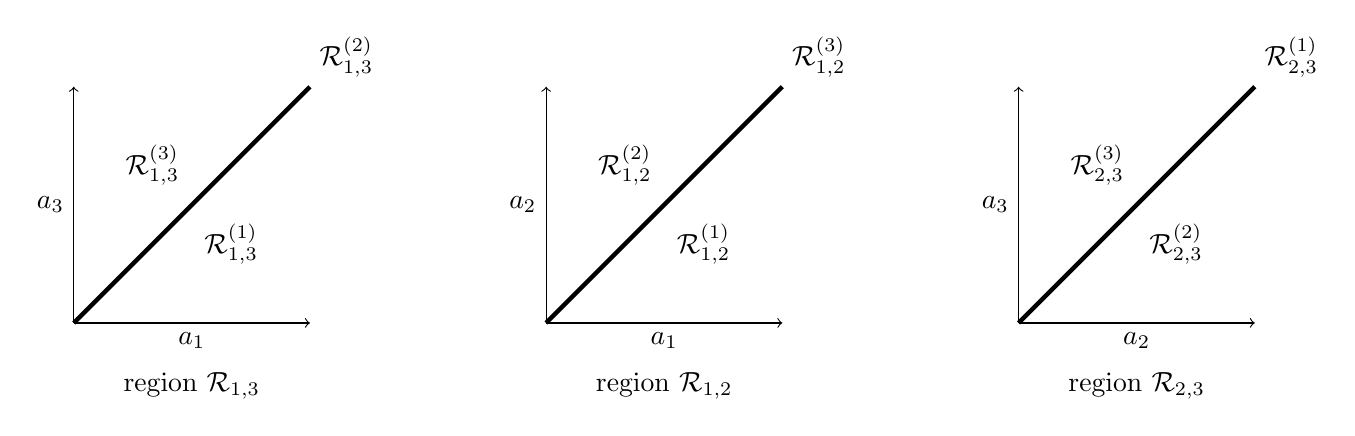
\begin{tikzpicture}
			
			
			
			\draw[->] (0,0)--(3,0);
			\draw[->] (0,0)--(0,3);
			\draw[ultra thick] (0,0)--(3,3);
			\node[below] at (1.5, 0){$a_1$};
			\node[left] at (0,1.5){$a_3$};
			\node at (1,2){$\mathcal{R}^{(3)}_{1,3}$};
			\node at (2,1){$\mathcal{R}^{(1)}_{1,3}$};
			\node [above right] at (3,3){$\mathcal{R}^{(2)}_{1,3}$};
			\node[below] at (1.5, -0.5){{\text region} $\mathcal{R}_{1,3}$};
			
			\draw[->] (6,0)--(9,0);
			\draw[->] (6,0)--(6,3);
			\draw[ultra thick] (6,0)--(9,3);
			\node[below] at (7.5, 0){$a_1$};
			\node[left] at (6,1.5){$a_2$};
			\node at (7,2){$\mathcal{R}^{(2)}_{1,2}$};
			\node at (8,1){$\mathcal{R}^{(1)}_{1,2}$};
			\node [above right] at (9,3){$\mathcal{R}^{(3)}_{1,2}$};
			\node[below] at (7.5, -0.5){{\text region} $\mathcal{R}_{1,2}$};
			
			\draw[->] (12,0)--(15,0);
			\draw[->] (12,0)--(12,3);
			\draw[ultra thick] (12,0)--(15,3);
			\node[below] at (13.5, 0){$a_2$};
			\node[left] at (12,1.5){$a_3$};
			\node at (13,2){$\mathcal{R}^{(3)}_{2,3}$};
			\node at (14,1){$\mathcal{R}^{(2)}_{2,3}$};
			\node [above right] at (15,3){$\mathcal{R}^{(1)}_{2,3}$};
			\node[below] at (13.5, -0.5){{\text region} $\mathcal{R}_{2,3}$};
			%%%%
		\end{tikzpicture}
\caption{At the left it is the region of $P_1,P_3$,  the middle  the region of $P_1,P_2$ and   the right  the region of $P_2,P_3$ } \label{region-1}
\end{center}
\end{figure}
%%%%%%%%%%%%%%%%%%%%%%%%%%%%%%%%





For $\nT^{(1)}$, $P_1$ is much smaller than $P_2$ and $P_3$. It means for 
\begin{equation}
\oint_{|P_1|=r_1} \oint_{|P_2|=r_2} \nd P_1 \wedge \nd P_2 \times \cdots  \, ,
\end{equation}
we have $r_1<|P_2|$. Hence $P_2=0$ and $P_3=0$ is not in the circle of $|P_1|=r_1$, but in the circle of $|P_2|=r_2$. That's why it does correspond to the contour $(\{P_1\},\{P_2,P_3\})$. One can also consider this problem starting from
\begin{equation}
\oint_{|P_1|=r_1} \oint_{|P_3|=r_2} \nd P_1 \wedge \nd P_3 \times \cdots  \, .
\end{equation}
and get the same conclusion. Similarly, one could know the contour of $\nT^{(2)}$ is $(\{P_2\},\{P_1,P_3\})$ and the contour of $\nT^{(3)}$ is $(\{P_3\},\{P_1,P_2\})$.

Now, as an exercise let's compute a multivariate residue  at $(0,0)$ of
\begin{equation}
\varphi=\frac{\left(z_1+z_2\right) R_{1,2}+z_2 R_{1,3}-z_1 R_{2,3}}{z_1 z_2 \left(z_1+z_2\right)}\nd z_1 \nd z_2 \, .
\end{equation}
For this simple case, the denominator of the rational function  can be directly separated to
\begin{equation}
\varphi=\frac{R_{1,2}}{P_1 P_2}\nd P_1 \wedge \nd P_2 + \frac{R_{1,3}}{P_1 P_3}\nd P_1 \wedge \nd P_3+\frac{R_{2,3}}{P_2 P_3}\nd P_2 \wedge \nd P_3 \, .
\end{equation}
Using the above analysis for the degenerated case, for the transformation $\nT^{(1)}$ we have 
%
\bea \varphi|_{\nT^{(1)}}={ (x_1^{(1)}+1) R_{1,2}+ R_{1,3}-x_1^{(1)} R_{2,3}\over x_1^{(1)}x_2^{(1)}(x_1^{(1)}+1) }
dx_1^{(1)}\wedge dx_2^{(1)} \, , \eea
%
thus
%
\bea \Res_{(0,0)} \nT^{(1)}[\varphi] = R_{1,2}+R_{1,3} \,. \eea
%
On the other side, from the analysis of contour, since the transformation $\nT^{(1)}$ corresponds to the contour $(\{P_1\},\{P_2 P_3\})$, $1/(P_1P_2)$ and $1/(P_1P_3)$ could contribute. Thus, the result is $R_{1,2}+R_{1,3}$. This result is the same as the one we get from transformation $\nT^{(1)}$. 
Similarly
\begin{align}
%&R^{(1)}=\Res_{(0,0)} \nT^{(1)}[\varphi] =+ R_{1,2}+R_{1,3} \nn\\
&R^{(2)}=\Res_{(0,0)} \nT^{(2)}[\varphi] = -R_{1,2}+R_{2,3}  \,,\nn\\
&R^{(3)}=\Res_{(0,0)} \nT^{(3)}[\varphi] = -R_{1,3}-R_{2,3} \, .
\end{align}
where the minus comes from $\nd P_i \wedge \nd P_j = -\nd P_j \wedge \nd P_i $. 
 $R^{(1)}+R^{(2)}+R^{(3)}=0$ is due to the three contours are not independent \cite{Larsen:2017aqb}.



Before ending this part, let us mention that there are other  transformations. For example, one could select $P_3$ as $x_1$ and $P_1$ as $x_2$, then, factorize a $x_2$ in the remaining degenerate factor $P_2$. This gives a factorization transformation
\begin{align}
&\nT^{(4)}: z_1\to x_2^{(4)}  \,,\  z_2\to x_1^{(4)}x_2^{(4)}-x_2^{(4)}\, .
\end{align}
which leads to 
%
\bea P_1=x_2^{(4)},~~~P_2=x_2^{(4)}(x_1^{(4)}-1),~~~~P_3=x_1^{(4)}x_2^{(4)} \, , ~~~\label{T4-1}\eea
%
and
\begin{align}
&\nT^{(4)}[u] =  \left(x_2^{(4)} \right)^{\beta_1 + \beta _2 + \beta_3} \left(x_1^{(4)}-1\right)^{\beta
   _2} 
 \left(x_1^{(4)}\right)^{\beta _3}  \times \cdots  \, , \nn\\
& \gamma^{(4)}_1=\beta_3 \,, \ \gamma^{(4)}_2=\beta_1+\beta_2+\beta_3  \, . ~~~\label{T4-2}
\end{align}
Comparing \eref{T4-1} with $\nT^{(3)}$ in \eref{T3-P}, we see they are same  after noting 
$P_1|_{\nT^{(3)}}\sim x_2^{(3)}$ and $P_2|_{\nT^{(4)}}\sim x_2^{(4)}$. 
Similarly, we have 
$\gamma^{(4)}_1 = \gamma^{(3)}_1$, $\gamma^{(4)}_2 = \gamma^{(3)}_2$ and $\mathcal{R}^{(4)} = \mathcal{R}^{(3)}$ by the analysis of region.
The  contour corresponds to $\nT^{(4)}[u]$ is also $(\{P_3\},\{P_1,P_2\})$, the same as $\nT^{(3)}$. These arguments show it is equivalent to the transformation $\nT^{(3)}$, thus we can neglect it. 

%%%%%%%%%%%%%%%%%%%%%%%%%%%%%%
\subsubsection{Region of factorization}
%%%%%%%%%%%%%%%%%%%%%%%%%%%%%%%%%

Now let's turn to a subtler issue about the power $b$ in the blow-up transformation \eqref{eq:Tblowup} for factorizing the
degenerated poles. The choice of $b$ relates also to the concept of "region" defined by the coordinate system of 
$a_i$, which describes the limit behavior $P_i\sim \lambda^{a_i}$. For the example presented in the previous subsubsection, the three factorization transformations $\nT^{(\alpha)}$ in \eref{3-T} are chosen such that
their sum of regions will fill the whole region defined by $\mathcal{R}_{i,j}=\{a_i>0,a_j>0\}$ for all pairs of $P_i=0,P_j=0$ as demonstrated in Figure~\ref{region-1}. We claim that only when the factorization transformation
satisfies this criterion, we will get the right  LO contribution using the formula \eref{eq:intnumdlog}.
Unfortunately, due to our limited mathematical knowledge, the rigorous mathematical reasons for this phenomenon are unclear to us. To reconfirm our calculations of the intersection numbers (such as the computations in section \ref{sec:eg2}) using the region method, we compute them again by the fibration algorithm \cite{Frellesvig:2019uqt} of multivariate intersection number. It is another algorithm that can compute multivariate intersection numbers but does not suffer from the complication of the multivariate complex function. 

Now let us illustrate some features of the subtler issue about blow-up transformation.
This problem arises from that we are not just computing the multivariate residue of a rational function, but also 
the residue of factorization transformation as the denominator in \eref{eq:intnumdlog}.
For a rational function, once it is factorized, further rescaling transformations will not change the result. For example
\begin{align}
\Res_{(0,0)}\frac{\nd z_1\wedge \nd z_2}{z_1 z_2} =1~~~~\label{res-1}
\end{align}
A further rescaling transformation\footnote{More generally, under the rescaling transformation 
$z_1\to t_1^a t_2^b,z_2\to t_1^c t_2^d$, the residue of \eref{res-1} is invariant when $ad-bc=1$. The blow-up transformations \eqref{eq:Tblowup} belong to the set of rescaling transformations.}
\begin{align}
\nT^{(1)}: z_1\to x^{(1)}_1 \left(x^{(1)}_2\right)^2\,, \ z_2\to x^{(1)}_2
\end{align}
will not change the result
\begin{align}
\Res_{(0,0)}\nT^{(1)}\left[\frac{\nd z_1\wedge \nd z_2}{z_1 z_2}\right] =\Res_{(0,0)}\frac{\nd x^{(1)}_1\wedge \nd x^{(1)}_2}{x^{(1)}_1 x^{(1)}_2} = 1 \, .
\end{align}
However,  the formula of LO contribution of intersection number \eref{eq:intnumdlog} contains the 
inverse of a residue in the denominator
\begin{align}
	\frac{1}{ \prod_{i} \Res_{\rho^{(\alpha)}_i} \partial_{z_i} \log\left(\nT^{(\alpha)}\left[u \right] \right) \nd z_i} \,
\end{align}
which will change under the rescaling transformations. 
For example, for  $u=z_1^{\beta_1}z_2^{\beta_2}\prod_{i=3}^n (\text{C}_i+\mathcal{O}(\bm{z}))^{\beta_i}$
which has been completely factorized, formula \eref{eq:intnumdlog} gives 
\begin{align}
\frac{1}{\bm{\gamma}} \equiv \frac{1}{ \prod_{i} \Res_{z_i=0} \partial_{z_i} \log u ~ \nd z_i} =\frac{1}{\beta_1 \beta_2}  \, .~~~\label{rescale-1-1}
\end{align}

Now we consider a rescaling transformation
\begin{align}
	\nT^{(1)}: z_1\to x^{(1)}_1 \left(x^{(1)}_2\right)^b \,, \ z_2\to x^{(1)}_2   ~~~\label{rescale-1-2}
\end{align}
such that 
\begin{align}
	&\nT^{(1)}[u] = \left(x^{(1)}_1\right)^{\beta_1}  \left(x^{(1)}_2\right)^{b\beta_1 + \beta_2}\prod_{i=3}^n (\text{C}_i+\mathcal{O}(\bm{z}))^{\beta_i} \nn\\
	&\frac{1}{\bm{\gamma}^{(1)}} =  \frac{1}{ \prod_{i} \Res_{\rho^{(\alpha)}_i} \partial_{z_i} \log\left(\nT^{(1)}\left[u \right] \right) \nd z_i} = \frac{1}{\beta_1(b\beta_1 + \beta_2)} \label{eq:overfactorized1}
\end{align}
Clearly, $1/\bm{\gamma} \neq 1/ \bm{\gamma}^{(1)}$, the further rescaling transformation will change the result of the intersection number. The reason is that before the rescaling transformation, the region is the complete first quadrant $\mathcal{R}_{1,2}=\{a_1>0,a_2>0\} $. After the rescaling transformation, we have 
%
\bea P_1=z_1= x^{(1)}_1 \left(x^{(1)}_2\right)^b,~~~~P_2=z_2=x^{(1)}_2 \eea
%
thus the region is given by 
$\mathcal{R}_{1,2}^{(1)}=\{a_1>ba_2>0\} $, which is only part of first quadrant. To get the right result, we must
sum up another rescaling transformation, which gives the region  $\mathcal{R}_{1,2}^{(1)}=\{ba_2>a_1>0\} $. One can see that such a rescaling transformation is given by 
\begin{align}
	\nT^{(2)}: z_1\to x^{(2)}_1  \,, \ z_2\to x^{(2)}_2\left(x^{(2)}_1\right)^{\frac{1}{b}}   
\end{align}
then
\begin{align}
	&\nT^{(2)}[u] = \left(x^{(2)}_1\right)^{\beta_1+\beta_2/b}  \left(x^{(2)}_2\right)^{\beta_2}\prod_{i=3}^n (\text{C}_i+\mathcal{O}(\bm{z}))^{\beta_i} \nn\\
	&\frac{1}{\bm{\gamma}^{(2)}} =  \frac{1}{ \prod_{i} \Res_{\rho^{(\alpha)}_i} \partial_{z_i} \log\left(\nT^{(2)}\left[u \right] \right) \nd z_i} = \frac{1}{(\beta_1 + \beta_2/b)\beta_2} \, .
\end{align}
It is easy to check that\footnote{More rigirously, there should be  a region $\mathcal{R}_{1,2}^{(1)}=\{ba_2=a_1>0\} $ to completely fill the complete first quadrant. However, the measure of this region is zero, so we can neglect it.}
\begin{align}
	\mathcal{R}_{1,2} = \mathcal{R}^{(1)}_{1,2} +\mathcal{R}^{(2)}_{1,2} \, , \quad \frac{1}{\bm{\gamma}} = \frac{1}{\bm{\gamma}^{(1)}} +\frac{1}{\bm{\gamma}^{(2)}}  \, .   \label{eq:regionrule}
\end{align}


Having the above example, we can come back to the example in the previous subsubsection for the degenerated pole. Let us keep 
factorization transformation of $\nT^{(1)}, \nT^{(2)}$ untouched, but change the factorizaton transformation of $\nT^{(3)}$. Again, in the first step, we do 
\begin{align}
	&{\text t}_1: z_1\to x_1-x_2\,, \ z_2\to x_2\, , \Longrightarrow 
	P_1=x_1-x_2\,,\ P_2=x_2\,,\  P_3=x_1\,.
\end{align}
But in the second step, we do 
\begin{align}
	&{\text t}_2: x_1\to x_1^{(3a)}(x_2^{(3a)})^b\,, ~~~\ x_2\to x_2^{(3a)}\, ,~~~b>1
\end{align}
Overall we have 
%
\bea  P_1=x_2^{(3a)}(x_1^{(3a)}(x_2^{(3a)})^{b-1}-1),~~~P_2=x_2^{(3a)},~~P_3=x_1^{(3a)} (x_2^{(3a)})^b~~~~\label{T3a-p}\eea
%
and
%
\bea & & \nT^{(3a)}[u] = \left(x_1^{(3a)}(x_2^{(3a)})^{b-1}-1\right)^{\beta
	_1}  \left(x_2^{(3a)} \right)^{\beta_1 + \beta _2 +b \beta_3} 
\left(x_1^{(3a)}\right)^{b\beta _3}  \times \cdots  \nnn
&&\gamma^{(3a)}_1=\beta_3 \,,\ ~~~~\gamma^{(3a)}_2=\beta_1+\beta_2+b\beta_3 \eea
%
It is easy to read out the region by $\nT^{(3a)}$ as 
%
\bea \mathcal{R}^{(3a)}_{1,2} = \{a_1=a_2>0\},~~~~\mathcal{R}^{(3a)}_{1,3} = \{a_3>ba_1>0\},~~~
\mathcal{R}^{(3a)}_{2,3} = \{a_3>b a_2>0\}\eea
%
If we check the Figure~\ref{region-1} again, we see that the region $\mathcal{R}_{1,3}$ and $\mathcal{R}_{2,3}$
is not complete. To find the missing region,  we need to consider another transformation
\bea
	&\widetilde{ {\text t}}_2:~~ x_1\to x_1^{(3b)}(x_2^{(3b)})^{1+{1\over b-1}}\,,~~~~ \ x_2\to x_1^{(3b)}(x_2^{(3b)})^{{1\over b-1}}\, 
\eea
Thus we have 
%
\bea P_1=x_1^{(3b)}(x_2^{(3b)})^{{1\over b-1}}(x_2^{(3b)}-1),~~~~P_2=x_1^{(3b)}(x_2^{(3b)})^{{1\over b-1}},~~~~P_3=x_1^{(3b)}(x_2^{(3b)})^{1+{1\over b-1}} \, , ~~~~\label{T3b-p}\eea
%
and 
%
\bea & & \nT^{(3b)}[u] = \left((x_2^{(3b)})-1\right)^{\beta
	_1}  \left(x_1^{(3b)} \right)^{\beta_1 + \beta _2 + \beta_3} 
\left(x_2^{(3a)}\right)^{\beta_1+\beta_2+b\beta_3\over b-1}  \times \cdots \,,  \nnn
&&\gamma^{(3b)}_1=\beta_1 + \beta _2 + \beta_3\,,\ ~~~~\gamma^{(3b)}_2={\beta_1+\beta_2+b\beta_3\over b-1}  \, . \eea
%
It is important to notice that both \eref{T3a-p} and \eref{T3b-p} gives the contour $\{ \{P_1,P_2\}, P_3\}$. Furthermore, from \eref{T3b-p} we find the region
%
\begin{equation}
\mathcal{R}^{(3b)}_{1,2} = \{a_1=a_2>0\},~~\mathcal{R}^{(3b)}_{1,3} = \{ba_1>a_3>a_1>0\},~
\mathcal{R}^{(3b)}_{2,3} = \{ba_2>a_3>a_2>0\} \, . 
\end{equation}
%
In fact, one can check that 
%
\bea & & {1\over \gamma^{(3a)}}+{1\over \gamma^{(3b)}}={1\over \beta_3(\beta_1+\beta_2+b\beta_3)}+{1\over (\beta_1 + \beta _2 + \beta_3)({\beta_1+\beta_2+b\beta_3\over b-1})}\nnn
%
& = & {1\over \beta_3(\beta_1+\beta_2+\beta_3)}={1\over \gamma^{(3)}}\eea
%
when compared with \eref{eq:examfactorize}.




We emphasize that the region rule is only observations in our practice, not proof. It suggests that if one does not want to lose contributions in this method, one should consider the regions of factorization transformations carefully.




%-------------------------------------------------


\subsection{The selection rules of the CDE---I}



With the above mathematical preparations, we move to the discussion of the matrix  $\big( \nds \Omega \big)$ 
defined in \eref{eq:intnumDE}. We will focus on the selection rules for non-zero components of $\big( \nds \Omega \big)$ by two different methods. In this section, we will discuss the computation 
of $\big( \nds \Omega \big)$ without using relative cohomology. Thus for denominators $D_i$ with integer power, we need to add a regulator  $D_i^{\delta_i}$ to $u$ and take the zero limit for the final result. As a consequence,  the selection rules of the CDE we get in this section will have some redundant terms, which will vanish together with the regulator power $\delta_i$. This problem will be avoided by using relative cohomology in the next
section. The discussion in this section will be the expansion of \cite{Chen:2023kgw}.
From \eref{eq:intnumDE} we see that the coefficient matrix of the CDE (or "CDE matrix" for short)  has two factors:
\begin{align}
	&\big( \nds \Omega \big)_{IK} = \braket{\dot{\varphi}_I|\varphi_J} \big( \eta^{-1} \big)_{JK} \, .
	\label{eq:intnumDE-1}
\end{align}
We will address these two factors one by one.
%---------------------------------

\subsubsection{Condition of $\braket{\dot{\varphi}_I|\varphi_J}\neq 0$}
%%%%%%%%%%%%%%%%%%%%%%%%%%%%%%%%%%%%%

Let's consider $\braket{\dot{\varphi}_I|\varphi_J}$ first. By general arguments, to have a non-zero contribution
to intersection number, one must have $b_{\dot{I},i}+b_{J,i} \leq -2$ for the series expansion around the pole $p_i$.
For $\varphi_J$ as a $\nd \log$-form, $b_{J,i}\geq -1$, thus only those terms in $\dot{\varphi}_I$ that satisfy $b_{\dot{I},i}\leq -1$ lead to non-zero contributions to this intersection number. Furthermore, around
each pole's region $(\alpha)$, the action of $\nds$ operator  decreases only one index $i$ of $b_{I,i}$
in the expansion of $\varphi_I$  by 1. Combining the fact that $\varphi_I$ is also a $\nd \log$-form, we have 
the condition: only when one index $j$ satisfies $b_{I,j}+b_{J,j}\leq -1$  and other indices satisfy  $b_{I,i}+b_{J,i} = -2, i\neq j$, $\braket{\dot{\varphi}_I|\varphi_J}$ could be non-zero.

With the above explanations, now we define two notations. For a pole's region $(\alpha)$, if they have a pair in the expansion which satisfy $b_{I,j}+b_{J,j} = -1$  and $b_{I,i}+b_{J,i} = -2$ for other  $i\neq j$, we say they share a {\bf $(n-1)$-variable Simple Pole (($n-1$)-SP)}; if  $b_{I,i}+b_{J,i} = -2$ for all $i$,  we say they share a {\bf $n$-SP}. Using these notations, the above discussions can be summarized as follows:
\begin{align}
&\begin{cases}
\nd \log \text{-form} &: \  b_{I,i}\geq-1 \, , \ b_{J,i}\geq-1 \, , \\
\dot{\varphi}_I &:\  b_{\dot{I},j} = b_{I,j}-1 \, , \ \text{for one $j$} \, , \\
\braket{\dot{\varphi}_I|\varphi_J}\neq 0 &: \ b_{\dot{I},i}+b_{J,i} \leq -2, ~\forall i 
\end{cases} \nn\\
&\Rightarrow \braket{\dot{\varphi}_I|\varphi_J}\neq 0 :\  (-2\leq b_{I,j}+b_{J,j} \leq -1) \  \& \  (b_{I,i}=b_{J,i} = -1, i\neq j)
\end{align}
and 
\begin{align}
\text{($n-1$)-SP} &: \ ( b_{I,j}+b_{J,j} = -1) \, \& \  (b_{I,i}=b_{J,i} = -1, i\neq j) \, , \nn\\
\text{$n$-SP} &:  \ b_{I,i}=b_{J,i} = -1 \, .
\end{align}

Before the computations of the above two cases, let us rewrite 
$\dot{\varphi}_I= \nD \log u \bigwedge_j \nD \log \nW^{(I)}_j$ given in \eref{tot-D} to more explicit form using the expansion \eref{eq:degenerate}
for factorization in the region $(\alpha)$ as  
\begin{align}
 &\nD \log \left( \nT^{(\alpha)} [u] \right) \bigwedge_j \nD \log \nT^{(\alpha)}\left[\nW^{(I)}_j \right] \, ,\nn\\
& \nD \log \left( \nT^{(\alpha)} [u] \right) = \nD \log \bar{u}_\alpha(\bm{x}^{(\alpha)}) + \nD \log \left(\prod_i \left[ x_i^{(\alpha)} - \rho_i^{(\alpha)} \right]^{\gamma_i^{(\alpha)}} \right) \,. \label{eq:TDlog}
\end{align}


%---------------------------------

\subsubsection{($n-1$)-SP contribution for $\braket{\dot{\varphi}_I|\varphi_J}$}


For $\varphi_I$ and $\varphi_J$ share a ($n-1$)-SP, $\nD \log \left( \nT^{(\alpha)} [u] \right)$ provides the remaining "one pole" via $b_{\dot{I},j}=b_{I,j}-1$.  The result is 
\begin{equation}
    -{\frac{{\gamma}^{(\alpha)}_j }{\bm{{\gamma}}^{(\alpha)}}} \, \nds \int C_{I}^{(\bm{b}_{I} )}C_J^{(\bm{b}_J)} \, d \rho^{(\alpha)}_j \,,
    \label{eq:NMCSPdlog}
\end{equation}
which has been given in \cite{Chen:2023kgw} (include why is it a $\nds \log$), so we are not going to explain these details again, but merely show one typical example: the $C_{I}^{(\bm{b}_{I} )}$ and $C_J^{(\bm{b}_J)}$ in the formula could be 
\begin{align}
&C_{I}^{(b_j=0)} = \left(\partial_{z} \log \tau[z,c_2;c_\pm] \right)\Big|_{z=c_1} = \partial_{c_1} \log \tau[c_1,c_2;c_\pm] \nn\\
&C_J^{(b_j=-1)}=\Res_{z=c_1} \nd \log \tau[z,c_1;c_\pm] =1  \, ,
\end{align}
then 
\begin{align}
\nds \int C_{I}^{(b_j=0)} C_J^{(b_j=-1)} \, d c_1 = \nds \log \tau[c_1,c_2;c_\pm]
\end{align}
Let us remind the reader that there are three cases for the $j$ in $b_{\dot{I},j}=b_{I,j}-1$:
\begin{align}
& b_{I,j}=0 \, , \ \ b_{J,j} = -1 \, , \nn\\
& b_{I,j}=-1 \, , \ \ b_{J,j} = 0 \, ,\nn\\
& b_{I,j}=-\frac{1}{2} \, , \ \ b_{J,j} = -\frac{1}{2} \, .
\end{align}
where the third case could emerge from sqrt-type $\nd \log$. According to the formula of LO contribution \eref{eq:LO}, $\tilde{\gamma}^{(\alpha)}_j$'s in the denominator rely on $b_{I,j}$ and $b_{J,j}$, and are different for these three cases. However, the $\nds$ act on $\int u \varphi_I$ also leads to a external factor $\tilde{\gamma}^{(\alpha)}_j$  at numerator.
For example, to use \eref{eq:intnumdlog}, we need to apply the rescaling transformation
\begin{align}
	\tilde{u} = u (z_j-\rho_j^{(\alpha)})^{-b_{I,j}} \, ,
\end{align}
and we have $\tilde{\gamma}^{(\alpha)}_i = \gamma^{(\alpha)}_i$  for $i\neq j$. 
Then, $\dot{\varphi}$ take the form as follow:
\begin{align}
	&~~~~\nds (z_j-\rho_j^{(\alpha)})^{\tilde{\gamma}^{(\alpha)}_j} \times \prod_{i\neq j}(z_i-\rho_i^{(\alpha)})^{\gamma^{(\alpha)}_i-1} f \nn\\
	&= -\tilde{\gamma}^{(\alpha)}_j \nds \rho_j^{(\alpha)} \times \prod_{i}(z_i-\rho_i^{(\alpha)})^{\tilde{\gamma}^{(\alpha)}_i-1} f + \cdots \, .
\end{align}
where the $\cdots$ part does not contribute to the intersection number. 
The $\tilde{\gamma}^{(\alpha)}_j$ in the above equation will cancel the $\tilde{\gamma}^{(\alpha)}_j$ in $\bm{\tilde{\gamma}}^{(\alpha)}$ in the equation \eref{eq:LO}:
\begin{equation}
	\frac{{\tilde{\gamma}}^{(\alpha)}_j }{\bm{{\tilde{\gamma}}}^{(\alpha)}}= \frac{1}{\prod_{i\neq j} \gamma^{(\alpha)}_i }  = \frac{\gamma^{(\alpha)}_j }{\bm{{\gamma}}^{(\alpha)}} \, .
\end{equation}
Hence, we have the coefficient in \eref{eq:NMCSPdlog}.


%---------------------------------

\subsubsection{$n$-SP contribution for $\braket{\dot{\varphi}_I|\varphi_J}$}

For $\varphi_I$ and $\varphi_J$ sharing a $n$-SP,  at first glance,  the second term  $\nD \log \left(\prod_i \left[ x_i^{(\alpha)} - \rho_i^{(\alpha)} \right]^{\gamma_i^{(\alpha)}} \right)$ in $\nD \log \left( \nT^{(\alpha)} [u] \right)$ (see \eref{eq:TDlog})  seems to lead to a pair of expanded terms that satisfy $b_{L,j}+b_{R,j}=-3$ for one $j$, and $b_{L,i}+b_{R,i}=-2$ for other $i\neq j$. 
This could give an NLO contribution (as defined in \cite{Chen:2023kgw}) to the intersection number. However, as we will show shortly, all these potential contributions are canceled here. For rational-type $\nd \log$-form,
\begin{equation}
\nD \log \nT^{(\alpha)}\left[\nW^{(I)}_j \right] = \nD \log \left(x_j^{(\alpha)}-\rho_j^{(\alpha)}\right)
\end{equation} 
expanding $D=\nds+\nd$ where  $\nds$ is differentiation with respect to $\rho_j^{(\alpha)}$ and $\nd_j$  differentiation with respect to $x_j^{(\alpha)}$, we have
\begin{align}
& ~\left[ \nd_{j} \log \left(\left( x_j^{(\alpha)} - \rho_j^{(\alpha)} \right)^{\gamma_j^{(\alpha)}} \right) 
\wedge \nds \log \left( x_j^{(\alpha)} - \rho_j^{(\alpha)} \right)  \right. \nn\\
&\left. ~ + \nds \log \left( \left( x_j^{(\alpha)} - \rho_j^{(\alpha)} \right)^{\gamma_j^{(\alpha)}} \right) 
\wedge \nd_j \log \left( x_j^{(\alpha)} - \rho_j^{(\alpha)} \right)  \right]   \bigwedge_{i\neq j}\nD \log \nT^{(\alpha)}\left[\nW^{(I)}_i \right]   \nn\\
= & \gamma_j^{(\alpha)} \left[ \nd_{j} \log \left( x_j^{(\alpha)} - \rho_j^{(\alpha)} \right)   
\wedge \nds \log \left( x_j^{(\alpha)} - \rho_j^{(\alpha)} \right) \right. \nn\\
&\left. ~~~~ + \nds \log \left( x_j^{(\alpha)} - \rho_j^{(\alpha)} \right)\wedge \nd_j \log \left( x_j^{(\alpha)} - \rho_j^{(\alpha)} \right)  \right]   \bigwedge_{i\neq j}\nD \log \nT^{(\alpha)}\left[\nW^{(I)}_i \right]   \nn\\
=&0 \, .
\end{align}
Similarly, for sqrt-type $\nd \log$-form 
\begin{equation}
\nD \log \nT^{(\alpha)}\left[\nW^{(I)}_j \right] = \nD \log \tau\left[x_j^{(\alpha)} ,\rho_j^{(\alpha)};c_{\pm} \right]
\end{equation} 
we have
\begin{align}
& ~\left[ \nd_{j} \log \left(\left( x_j^{(\alpha)} - \rho_j^{(\alpha)} \right)^{\gamma_j^{(\alpha)}} \right) \wedge \nds \log \tau\left[x_j^{(\alpha)} ,\rho_j^{(\alpha)};c_{\pm} \right]  \right. \nn\\
&\left. +  \nds \log \left(\left( x_j^{(\alpha)} - \rho_j^{(\alpha)} \right)^{\gamma_j^{(\alpha)}} \right) \wedge \nd_j \log \tau\left[x_j^{(\alpha)} ,\rho_j^{(\alpha)};c_{\pm} \right]   \right] 
\bigwedge_{i\neq j}\nD \log \nT^{(\alpha)}\left[\nW^{(I)}_i \right]   \nn\\
=& \left[ \nd_{j} \log \left( x_j^{(\alpha)} - \rho_j^{(\alpha)} \right)\wedge \nds \log \left( x_j^{(\alpha)} - \rho_j^{(\alpha)} \right)  + \nds \log \left( x_j^{(\alpha)} - \rho_j^{(\alpha)} \right)\wedge \nd_j \log \left( x_j^{(\alpha)} - \rho_j^{(\alpha)} \right)  \right] \nn\\
&  \times \frac{\gamma_j^{(\alpha)} \sqrt{\left(\rho_j^{(\alpha)}-c_+\right) \left(\rho_j^{(\alpha)}-c_-\right)}   }{ \sqrt{\left(x_j^{(\alpha)}-c_+ \right) \left(x_j^{(\alpha)}-c_- \right)} }  
\bigwedge_{i\neq j}\nD \log \nT^{(\alpha)}\left[\nW^{(I)}_i \right]   \nn\\
=&0
\end{align}

After showing the second term giving no contribution, using the result \eref{eq:LO} the first term  gives the
result
\be
\frac{C_I^{(\bm{-1})} C_J^{(\bm{-1})}}{\bm{\gamma}^{(\alpha)}} \, \nds \log \Big( \bar{u}_\alpha(\bm{\rho}^{(\alpha)}) \Big) \,.  \label{eq:CSPdlog}
\end{equation}
It is worth pointing out that 
in \cite{Chen:2023kgw}, one needs a formula of the NLO contribution of the intersection number for this result. Here we avoid using the NLO formula because we have transformed the related term to the LO case via IBP in  \eref{eq:Dlogvarphi} 
(from the second line to the third line) at the beginning.


%------------------------------------------------

\subsubsection{Condition of $\big( \eta^{-1} \big)_{JK}\neq 0$}
For $\big( \eta^{-1} \big)_{JK}$  in the CDE, since $\eta^{-1}={1\over |\eta|}\eta^*$ where $\eta^*$ is the adjugate matrix, the element could be written as 
\begin{equation}
\big( \eta^{-1} \big)_{JK} = (-1)^{J+K} \frac{\eta^{(KJ)}}{|\eta|}
\end{equation}
where $\eta^{(KJ)}$ is the minor of the element $\eta_{JK}$ in the matrix  $\eta$. The minor in the Laplace expansion of the determinant is the sum of the form
%
\begin{equation}
	(-1)^a \eta_{J i_1}\eta_{i_1 i_2}\cdots \eta_{i_{v-1} i_v}\eta_{i_v K} \prod_{k}\eta_{j_k j_k} \, .~~\label{eta-form}
\end{equation}
%
For $\eta^{(KJ)}\neq 0$, at least one term of the form \eref{eta-form} should be non-zero, which 
is equivalent to the statement that every element $\eta_{ij}$ in \eref{eta-form} should be non-zero. For the $\nd \log$-form
$\eta_{JK} = \braket{\varphi_J|\varphi_K}$ could be non-zero only when  $\varphi_J$ and  $\varphi_K$ share at least one $n$-SP. Since 
 $\varphi_{j_k}$ must exhibit $n$-SP with itself, all $\eta_{j_k j_k}$ should naturally be non-zero. Therefore, we only need to ask  the existence of at least one non-zero chain $\eta_{J i_1}\eta_{i_1 i_2}\cdots \eta_{i_{v-1} i_v}\eta_{i_v K}$, which implies that $\varphi_J$ shares $n$-SP with $\varphi_{i_1}$, $\varphi_{i_1}$ shares $n$-SP with $\varphi_{i_2}$, and so on. With this picture, the notation of 
{\bf  $n$-SP chain} has been defined  in \cite{Chen:2023kgw}: 
\begin{itemize}
\item If $\varphi_I$ and $\varphi_J$ share an $n$-SP, we say they are $n$-SP related, and denote it as $\varphi_I \sim \varphi_J$. 
\item The $n$-SP chain is the collection of $\varphi_I$'s, such that for arbitrary pair of $\varphi_a, \varphi_b$
there exists an ordered list $\{\varphi_a, \varphi_{i_1},...,\varphi_{i_k}, \varphi_b \}$ (notice that $\varphi_a\sim \varphi_b, \varphi_b \sim \varphi_c$ do not give $\varphi_a \sim \varphi_c$, that is why there is a order) such that
$\varphi_a\sim \varphi_{i_1}\sim ...\sim \varphi_{i_k}\sim\varphi_b $ where every $\varphi$ belongs to the chain.  If $\varphi_a, \varphi_b$ belong to a $n$-SP chain, we denote it as $\varphi_a\sim\sim\varphi_b$. 

\end{itemize}
Using this notation, we can simply say that the  condition of $\big( \eta^{-1} \big)_{JK}\neq 0$  is  $\varphi_J$ and $\varphi_K$ belongs to an $n$-SP chain.
For example, assume there is a case with seven master integrals, whose indices are denoted as $\{J,K,1,2,3,4,5\}$,  and suppose $\varphi_J\sim\varphi_1\sim\varphi_2\sim\varphi_K$, we have  $\varphi_J\sim\sim\varphi_K$ and 
\begin{equation}
(-1)^{J+K}|\eta^{(KJ)}| = \left|
\begin{array}{cccccc}
 * & \eta _{J1} & * & * & * & *
   \\
 * & * & \eta _{12} & * & * & * \\
 \eta _{2K} & * & * & * & * & * \\
 * & * & * & \eta _{33} & * & * \\
 * & * & * & * & \eta _{44} & * \\
 * & * & * & * & * & \eta _{55} \\
\end{array}
\right|
\end{equation}
could be non-zero due to $\eta _{\text{J}1}\eta _{12}\eta _{2\text{K}}\eta _{33}\eta _{44}\eta _{55}$ could be non-zero.

%-------------------------------------------------------

\subsubsection{Conclusion}

Having discussed the two factors in \eref{eq:intnumDE}, now we can state the selection rules of the CDE:
\begin{itemize}
\item $\big( \nds \Omega \big)_{IK} = \braket{\dot{\varphi}_I|\varphi_J} \big( \eta^{-1} \big)_{JK}$ could be non-zero only when in the summation over $J$ there exists a $\varphi_J$ share ($n-1$)-SP or $n$-SP with $\varphi_I$, and $\varphi_J\sim\sim\varphi_K$.
\item $\big( \nds \Omega \big)_{IK}$ could be determined via merely LO contribution formula of intersection number. For $\varphi_I$ and $\varphi_J$ that share a  ($n-1$)-SP, it contributes
\begin{equation}
    -{\frac{{\gamma}^{(\alpha)}_j }{\bm{{\gamma}}^{(\alpha)}}} \, \nds \int C_I^{(\bm{b}_I)}C_J^{(\bm{b}_J)} \, \nds \rho^{(\alpha)}_j \,
    \label{eq:NMCSPdlog1}
\end{equation}
to $\braket{\dot{\varphi}_I|\varphi_J}$. For $\varphi_I$ and $\varphi_J$ share a  $n$-SP, it contributes
\begin{equation}
\frac{C_I^{(\bm{-1})} C_J^{(\bm{-1})}}{\bm{\gamma}^{(\alpha)}} \, \nds \log \Big( \bar{u}_\alpha(\bm{\rho}^{(\alpha)}) \Big) \,.  \label{eq:CSPdlog1}
\end{equation}
to $\braket{\dot{\varphi}_I|\varphi_J}$ with constant $C_I^{(\bm{-1})} C_J^{(\bm{-1})}$. These two formulas give all symbol letters. For $\eta_{JK}=\braket{\varphi_J|\varphi_K}$, each shared $n$-SP gives
\begin{equation}
 \frac{C_J^{(\bm{-1})} C_K^{(\bm{-1})}}{\bm{\gamma}^{(\alpha)}}  \label{eq:inveta}
\end{equation}
with constant $C_J^{(\bm{-1})} C_K^{(\bm{-1})}$.

\item The canonical-form differential equations emerge naturally. 
To see it, let's assign the original hypersurface-powers $\beta_i$ in $u=\prod_i \left[P_i(\bm{z})\right]^{\beta_i}$ to  have the transcendental weight-($-1$). For our application in Feynman integrals, $\beta_i\sim a  \ep$ or $\beta_i \sim \delta_k$ with constant $a$ (typically, integer or half-integer). This means that $\ep$ and $\delta_i$ have the transcendental weight-($-1$), so all hypersurface-powers $\gamma^{(\alpha)}_i$ for each factorization are also weight-($-1$)
\begin{equation}
\mathcal{T}(\beta_i) = \mathcal{T}(\ep) = \mathcal{T}(\delta_k) = \mathcal{T}(\gamma^{(\alpha)}_i) = -1\, .
\end{equation}
Because of \eref{eq:NMCSPdlog1} and \eref{eq:CSPdlog1}, $\braket{\dot{\varphi}_I|\varphi_J}$ are weight-($n$-$1$) coefficient times $\nds \log$-form. Similarly,  $\big( \eta^{-1} \big)_{JK}$
is weight-($-n$) coefficient. Combining them, we have $\big( \nds \Omega \big)_{IK}$ is weight-($-1$) coefficient times $\nds \log$-form.  After taking regulators $\delta_i$ to  zero, the weight-($-1$) coefficient in $\big( \nds \Omega \big)_{IK}$ could only be proportional to $\ep$. Hence we have 
\begin{equation}
\big( \nds \Omega \big)_{IK} = \ep \sum_i \text{C}^{(i)}_{IK} ~ \nds \log \text{W}^{(i)}(\bm{s}) \label{eq:CDE}
\end{equation}
where $\text{W}^{(i)}(\bm{s})$ are symbol letters and $\text{C}^{(i)}_{IK}$ are the corresponding  constant coefficient matrix. This is nothing, but the so-called canonical form or $\ep$-form.
\end{itemize}
Since after factorization, the n-variable multivariate residues are reduced to n univariate residues, and only the ($n_0\geq$  $n-1$)-SP shared by $\varphi_I$ and $\varphi_J$  could contribute, naturally one can image that people could take residue of $(n-1)$-SP first. This gives an overall factor  
\begin{equation}
{\frac{{\gamma}^{(\alpha)}_j }{\bm{{\gamma}}^{(\alpha)}}}
\end{equation}
and left an univariate problem, whose u part (denoted as $u'$ here) is
\begin{equation}
u'=\bar{u}_\alpha(\rho_1^{(\alpha)},\cdots,\rho_{j-1}^{(\alpha)}, x_j^{(\alpha)},\rho_{j+1}^{(\alpha)},\cdots,\rho_{n}^{(\alpha)} ) \left( x_j^{(\alpha)} - \rho_j^{(\alpha)} \right)^{\gamma_j^{(\alpha)}}
\end{equation}
All univariate u-part could be reformed as 
\begin{equation}
u' =P_0^{\beta_0} \prod_i (z-c_i)^{\beta_i} \,.
\end{equation}
Since we rescale all $\beta_i$ to be $a_i \ep$, the square root part is absorbed into $\bar{\varphi}$ part. Without loss of generality, the square root part can be expressed as $\prod_{i=1}^{m}(z-c_i)^{-\frac{1}{2}}$. For the cases we discussed in this paper, $m=0,1,2$, so that there is no elliptic integral and it is the $\nd \log$ cases. If $m=3,4$, they are the elliptic cases. If $m\geq 5$, it is the beyond elliptic case.
Then, the $\nd \log$ basis and the CDE of all univariate cases without elliptic integrals ($m=0,1,2$) could be systematically discussed based on this form and of course give the same answer as \eref{eq:NMCSPdlog1} and \eref{eq:CSPdlog1}. The details of the univariate $\nd \log$ cases have been given in \cite{Chen:2023kgw}. \cite{Chen:2023kgw} also shows that since univariate rationalization is easy, one could also transform all $m=0,1,2$ cases into the $m=0$ cases with an algebraic transformation. Let's denote the new $u$ after the transformation as 
\begin{equation}
u'=(P_0')^{a_0 \ep} \prod_i (z'-c_i')^{a_i \ep} \,.
\end{equation}
Then, all the symbol letters are the distance between these univariate poles $c_i'-c_j'$ and pure parameter factor $P_0'$ as has been discussed in \cite{Chen:2023kgw}. For the $m\geq 3$ cases, which are elliptic or beyond, unfortunately, there are not a $\nd \log$ basis then. Meanwhile, the square roots like $\prod_{i=1}^{3}(z-c_i)^{-\frac{1}{2}}$ can not be rationalized by an algebraic transformation. These cases are beyond the scope of this paper.

%--------------------------------------------------

\section{The selection rules of the CDE via relative cohomology} \label{sec:RC}


\subsection{Dual form in twisted relative cohomology}
In the last section, we have introduced how to compute the intersection number between forms in twisted cohomology. In this section, we will 
present simple computational rules for intersection numbers between twisted cohomology and twisted relative cohomology. 
Recall the integrals take the form
\begin{align}
&I[u,\varphi] \equiv \int  u \, \varphi_L  \,,   \nn \\
&\varphi \equiv \hat{\varphi}(\bm{z}) \bigwedge_j \nd z_j =\frac{Q(\bm{z})}{\left(\prod_k D_k^{a_k} \right) \left(\prod_i P_i^{b_i} \right)} \bigwedge_j \nd z_j \, , \nn\\
&u=\prod_i \left[P_i(\bm{z})\right]^{\beta_i} \,,
    \quad \quad  a_k, b_j\in \mathbb{N}  \, ,
    \label{eq:baikov1}
\end{align}
where regulators have not been introduced for factors $ D_k$.  
In Feynman integrals, the  denominators $D_i$ with integer power are propagators and determine the “sector" to which the integral belongs to. Here we borrow the concept of "sector" from the Feynman integral by considering  denominators in $\varphi_I$ having negative integer power in $u\varphi_I$\footnote{The $P_i$ in $\varphi_I$  will have contribution from $u$, so the total power is not integer and we should consider them as the "propagator". }
as the "propagator" and defining the sector by the list $\hat{I}$ selecting from the set of propagators. Furthermore, we denote the set of hypersurfaces relating to the sector $\hat{I}$ as  
\begin{equation}
\mathcal{B}_{\hat{I}} = \{D_{I_1}=0,D_{I_2}=0,\cdots,D_{I_n}=0  \} \, . ~~~\label{B-cut}
\end{equation}
Selecting the dual space of dual form $\ket{\varphi}$ to be the space of twisted  relative cohomology just means selecting  dual forms living on the maximal cut of each sector. To distinguish, we denote these dual forms living on its maximal cut $(\hat{R})$ as $\Delta_{\hat{R}}\varphi_R$. In practice, we do not need to know the exact meaning of "live on the cuts", and all we need to know is the intersection number of $\varphi_L$ and $\Delta_{\hat{R}}\varphi_R$ obey a simple rule: just applying the maximal cut of the sector of $\varphi_R$ to both sides, then applying the intersection number between the cut forms as we did in the previous section, i.e.,
\begin{align}
&\braket{\varphi_L|\Delta_{\hat{R}}\varphi_R}= \braket{\varphi_{L;\hat{R}}  |\varphi_{R;\hat{R}}} = \sum_{\bm{p}_{\hat{R}}}\Res_{\bm{p}_{\hat{R}}=0} \psi_{L;\hat{R}} \varphi_{R;\hat{R}}   \, , \quad \nabla_{1;\hat{R}} \cdots \nabla_{n;\hat{R}} \psi_{L;\hat{R}} = \varphi_{L;\hat{R}} \nn\\
& \varphi_{L;\hat{R}} = \Res_{\mathcal{B}_{\hat{R}}}  \left( \frac{u\varphi_L}{u_{\hat{R}}}\right)  \, , \quad  \varphi_{R;\hat{R}} = \Res_{\mathcal{B}_{\hat{R}}}  \left( \frac{\varphi_R u_{\hat{R}}}{u} \right)      \, , \quad  u_{\hat{R}}=u|_{\mathcal{B}_{\hat{R}}} \, , ~~~\label{3.3}
\end{align}
where $\nabla_{i;\hat{R}}$  is defined via the cut integral family corresponding to $u_{\hat{R}}$.  $\bm{p}_{\hat{R}}$ are again isolated intersection points (see \eref{eq:intnum}) of hypersurfaces
containing  $\mathcal{B}_{\hat{R}}$. The definition of $\varphi_{L;\hat{R}}$ in \eref{3.3} has the property
$\Res_{\mathcal{B}_{L;\hat{R}}}  u \varphi = u_{\hat{R}} ~ \varphi_{L;\hat{R}}$, and the form in \eref{3.3}
makes $\varphi_{L;\hat{R}}$ manifest as the single-valued function. 







In relative cohomology, the concept of "subsector" is the same as Feynman integrals, i.e., if $\mathcal{B}_{\hat{I}}  \subseteq \mathcal{B}_{\hat{J}} $, we say $\mathcal{B}_{\hat{I}}$ is a subsector of $\mathcal{B}_{\hat{J}}$. Obviously, only when the sector of $\varphi_R$ is a subsector of the sector of $\varphi_L$, the intersection number could be non-zero.




\subsection{The improved selection rules of the CDE}

Now we consider the $\nds \Omega$ in the CDE using the dual basis in the relative cohomology
\begin{align}
    &\big( \nds \Omega \big)_{IK} = \braket{\dot{\varphi}_{I;\hat{J}}|\varphi_{J;\hat{J}}} \big( \eta^{-1} \big)_{JK} \, ,\nn\\
    & \eta_{IJ}\big( \eta^{-1} \big)_{JK} = \delta_{IK}   \, , \ \         \eta_{IJ} = \braket{\varphi_{I;\hat{J}}|\varphi_{J;\hat{J}}} .
    \label{eq:intnumDEc}
\end{align}
For $\braket{\dot{\varphi}_{I;\hat{J}}|\varphi_{J;\hat{J}}}$, let us denote the number of remaining integration variables of sector $\mathcal{B}_{\hat{J}}$ as $n_{\hat{J}}$. With the knowledge discussed in the previous section, we see immediately that  $\braket{\dot{\varphi}_{I;\hat{J}}|\varphi_{J;\hat{J}}}$ could be non-zero only when $\dot{\varphi}_{I;\hat{J}}$ and $\varphi_{J;\hat{J}}$ share $n_{\hat{J}}$-SP or ($n_{\hat{J}}-1$)-SP.

For $\big( \eta^{-1} \big)_{JK}$, things are a little bit different since
$\braket{\varphi_{I;\hat{J}}|\varphi_{J;\hat{J}}}\neq \braket{\varphi_{J;\hat{I}}|\varphi_{I;\hat{I}}}$. 
To count the anti-symmetry, we need to slightly modify the concept of $n$-SP chain to a new concept of {\bf cut-$n$-SP} chain, i.e.,
\begin{itemize}
\item If ${\varphi}_{I;\hat{J}}$ and $\varphi_{J;\hat{J}}$ share $n_{\hat{J}}$-SP,  we say $\varphi_I$ is cut-$n$-SP related to $\varphi_J$, and denoted as $\varphi_I \rightarrow \varphi_J$ or $\varphi_J \leftarrow \varphi_I$. Now, it is an oriented relation, i.e., $\varphi_I \rightarrow \varphi_J$ does not imply $\varphi_J \rightarrow \varphi_I$. %"Maximal" for $\dot{\varphi}_{I;\hat{J}}$ and $\varphi_{J;\hat{J}}$ are  $n_{\hat{J}}$-forms and share $n_{\hat{J}}$-SP.

\item If $\varphi_I \rightarrow \varphi_J$, we also say that $\varphi_I$ is linked to $\varphi_J$ via a cut-$n$-SP chain. If $\varphi_I \rightarrow \varphi_J$ and $\varphi_J \rightarrow \varphi_K$, then we say $\varphi_I$ is linked to $\varphi_K$ via the cut-$n$-SP chain $\varphi_I \rightarrow \varphi_J \rightarrow \varphi_K$, we denote it as $\varphi_I \rightarrow\rightarrow \varphi_J$. Similar understanding for more forms $\varphi$.  
\end{itemize}
With the above definition the condition of $\big( \eta^{-1} \big)_{JK}$ could be non-zero is  $\varphi_J \rightarrow\rightarrow \varphi_K$. Obviously, if  $\mathcal{B}_{\hat{I}}  \subset \mathcal{B}_{\hat{J}}$, $\varphi_I \rightarrow \rightarrow \varphi_J$ could not be true.

The contributions for $\braket{\dot{\varphi}_{I;\hat{J}}|\varphi_{J;\hat{J}}}$  are still calculated via \eref{eq:NMCSPdlog1} and \eref{eq:CSPdlog1}. However, every element in these expressions should be replaced by the cut one, corresponding to the maximal cut  $\mathcal{B}_{\hat{J}}$. One difference the cut leads to is the transcendent weight of coefficient $\gamma^{(\alpha)}_j/\bm{\gamma}^{(\alpha)}$,  which changes from $n-1$ to   $n_{\hat{J}}-1$. Similarly, contributions for $\left(\eta^{-1}\right)_{JK}$ is calculated via \eref{eq:inveta}, but the weight of coefficient becomes $-n_{\hat{J}}$. One point that needs to be emphasized is that
since we avoid regulators at the beginning, only $a \ep$ appears in $\beta_i$ and hypersurface-powers.  Weight-n coefficient could only be proportional  to $\ep^{-n}$.


With the above discussions,  we have the selection rules of the CDE (improved and exact version):
\begin{itemize}
\item $\big( \nds \Omega \big)_{IK} = \braket{\dot{\varphi}_{I;\hat{J}}|\varphi_{J;\hat{J}}} \big( \eta^{-1} \big)_{JK}$ could be non-zero only when there exist at least one $\varphi_J$ that $\dot{\varphi}_{I;\hat{J}}$ and $\varphi_{J;\hat{J}}$ share $n_{\hat{J}}$-SP or ($n_{\hat{J}}-1$)-SP  and $\varphi_J \rightarrow \rightarrow \varphi_K$.

\item $\big( \nds \Omega \big)_{IK}$ could be determined via merely LO contribution formula of intersection number. It gives cut version of \eref{eq:NMCSPdlog1} and \eref{eq:CSPdlog1} for $n_{\hat{J}}$-SP or ($n_{\hat{J}}-1$)-SP contribution in $\braket{\dot{\varphi}_{I;\hat{J}}|\varphi_{J;\hat{J}}}$ and cut vertion of \eref{eq:inveta} for $\left(\eta^{-1}\right)_{JK}$.
 
\item  $\braket{\dot{\varphi}_{I;\hat{J}}|\varphi_{J;\hat{J}}} \big( \eta^{-1} \big)_{JK}$ is  weight-($-1$) coefficient, which could only be propotional to $\ep$, times  $\nds \log$-form. Thus canonical differential equation emerges.
\end{itemize}

We know that the differential of a Feynman integral belonging to a subsector will not rely on a higher sector, so
\begin{align}
\text{If } \mathcal{B}_{\hat I} \subset \mathcal{B}_{\hat K}\, , \ \text{then } \nds \Omega_{IK} = 0  \, .  \label{eq:relyonsub}
\end{align}
Unfortunately, with regulators the structure of the sector has been broken, i.e., there is also no explicit reason to tell us if $\mathcal{B}_{\hat I} \subset \mathcal{B}_{\hat K}$. Thus the statement \eref{eq:relyonsub} is not true and  $\nds \Omega_{IK}$  vanishes when and only when taking regulators to  zero after the computation of intersection number. This is one of the manifestations of redundancy when using the regulator method.
However, with dual form in relative cohomology,  $\braket{\dot{\varphi}_{I;\hat{J}}|\varphi_{J;\hat{J}}}$ could be non-zero only when $\mathcal{B}_{\hat{J}} \subseteq \mathcal{B}_{\hat{I}}$. Furthermore, $(\eta^{-1})_{JK}$ could be non-zero only when $\mathcal{B}_{\hat{K}} \subseteq \mathcal{B}_{\hat{J}}$. Therefore, $\big( \nds \Omega \big)_{IK}$ could be non-zero only when $\mathcal{B}_{\hat{K}} \subseteq \mathcal{B}_{\hat{I}}$ and \eref{eq:relyonsub} holds true as well.






%------------------------------------------------
%--------------------------------------------------

\section{Univariate example: $u=z^\delta (z-c_1)^\ep(z-c_2)^\ep$} \label{sec:eg1}

In this section, we consider the case $u=z^\delta (z-c_1)^\ep(z-c_2)^\ep$, where $\delta$ is a regulator. This structure appears in many cases of Feynman integral. For example, all n-point one-loop integrals with their $n-1$ propagator cut will give such a $u$ in their Baikov representation. We will compute its CDE via both methods, with and without regulators. 

For the given $u$, the related hypersurfaces are
\begin{align}
\mathcal{B}=\{z=0,z-c_1=0,z-c_2=0,z=\infty\} \,.
\end{align}
Its $\nd \log$ basis can be easily constructed as
\begin{align}
\varphi_1 = \frac{\nd z}{z} =\nd \log z \, ,  \quad \varphi_2 = \frac{\nd z}{z-c_1} - \frac{\nd z}{z-c_2}  = \nd \log \left( \frac{z-c_1}{z-c_2}\right)  \, .
\end{align}

%------------------------------------
\subsection{With regulator}
With a regulator, we have
\begin{align}
\omega=\nd \log u = \left( \frac{\delta}{z} + \frac{\ep}{z-c_1}+ \frac{\ep}{z-c_2} \right) \nd z \, .
\end{align}
Poles of $\omega$ are
\begin{align}
\{\bm{p}\}=\{0,c_1,c_2,\infty\} \, 
\end{align}
and the hypersurface powers corresponding to each pole are
\begin{align}
\gamma_1=\delta\, , \ \ \gamma_2=\ep\, , \ \ \gamma_3=\ep\, , \ \ \gamma_4=-2\ep-\delta \, .
\end{align}
Now we compute $\eta_{IJ}=\braket{\varphi_I|\varphi_J}$ using the result \eref{eq:intnumexpand} and \eref{eq:LO}. 
For $\eta_{11}$,  $\varphi_1$ shares 1-SP with itself at the points $0$ and $\infty$. For $\eta_{12}$,
$\varphi_1$ do not share any pole with $\varphi_2$. For  $\varphi_2$, it  shares 1-SP with itself at the points $c_1$ and $c_2$.  Thus we have  we have 
\begin{align}
&\eta=\braket{\varphi_I|\varphi_J}=\left(
\begin{array}{cc}
 \frac{1}{\gamma_1}+\frac{1}{\gamma_4} & 0 \\
 0 &  \frac{1}{\gamma_2}+\frac{1}{\gamma_3}  \\
\end{array}
\right)=\left(
\begin{array}{cc}
 \frac{1}{\delta }-\frac{1}{\delta +2 \epsilon } & 0 \\
 0 & \frac{2}{\epsilon } \\
\end{array}
\right)  \, , \nn\\
&\eta^{-1}=\left(
\begin{array}{cc}
 \delta(\delta+2\ep)/(2 \epsilon)  & 0 \\
 0 & \epsilon/2 \\
\end{array}
\right)  \, .
\end{align}
Let's turn to consider $\braket{\dot{\varphi}_I|\varphi_J}$. Using \eref{eq:Dlogvarphi} we have $\dot{\varphi}_I$
\begin{align}
&\dot{\varphi}_1 = \nD \left(\log \bar{u}_1(z) + \delta \log z \right) \wedge \nD \log z \nn\\
& \quad = \nD \log \bar{u}_1(z) \wedge \nD \log z= \nd \log \bar{u}_1(z) \wedge \nds \log z+\nds \log \bar{u}_1(z) \wedge \nd \log z \, , \nn\\
&\dot{\varphi}_2 =  \nD \log \bar{u}_2(z) \wedge \nD \log (z-c_1) - \nD \log \bar{u}_3(z) \wedge \nD \log (z-c_2)   \nn\\
&\quad = \delta ~ \nD \log z \wedge \varphi_2 + 2 \ep ~ \nD \log (z-c_2) \wedge \nD \log (z-c_1)  \, . ~~~\label{4.7}\end{align}
As a reminder, the $\nds$ here is a formal differential operator with respect to arbitrary one parameter. Since it could act on $c_1$ as well as  $c_2$, we should keep both $\nds \log (z-c_1)$ and $\nds \log (z-c_2)$. Notice that even for $\nds \log z$, we still keep it, because  we regard $\nds \log z$ as $\nds \log (z-c_0)$ with $c_0=0$ and $\nds$ could act on $c_0$ as well.
In \eqref{4.7}, the $\bar{u}_i(z)$ is defined in \eref{eq:degenerate-1} and for current example they are 
%
\bea 
\bar{u}_1(z) = (z-c_1)^\ep(z-c_2)^\ep \, ,  
\bar{u}_2(z) = z^\delta(z-c_2)^\ep \, ,
\bar{u}_3(z) = z^\delta(z-c_1)^\ep \, . 
\eea
As a pedagogical example, we show the computation details of  $\braket{\dot{\varphi}_1|\varphi_1}$ here. 
First as the d-log form, $\varphi_1$ shares 1-SP with itself only, i.e., there is no contribution from 
0-SP. For 
pole $z=0$, the first term of $\dot{\varphi}_1$ in \eref{4.7}  gives zero contribution, while the second term gives the contribution
\begin{align}
\frac{1}{\delta} \nds \log \left((z-c_1)^\ep(z-c_2)^\ep|_{z=0} \right) = \frac{\ep}{\delta} \nds \log(c_1c_2)  \,,
\end{align}
For the pole $z=\infty$ the second term gives the contribution
\begin{align}
\frac{1}{-\delta-2\ep} \nds \log \left((1-c_1 t)^\ep(1-c_2 t)^\ep|_{t=0} \right) = \frac{\ep}{-\delta-2\ep} \nds \log 1 = 0 \,,
\end{align}
where $t=1/z$. %Thus it has no contribution.
For $\braket{\dot{\varphi}_1|\varphi_2}$, $\varphi_1$ shares the 0-SP with $\varphi_2$ at the poles $c_1,c_2$. The contribution is $\nds \log
\left(c_2/c_1\right) $, which   can be seen from the first term  of $\dot{\varphi}_1$ in \eref{4.7}. After finishing all these computations,  we have 
\begin{align}
\Big( \braket{\dot{\varphi}_I|\varphi_J} \Big) = \nds \left(
\begin{array}{cc}
 \frac{\epsilon }{\delta } \log \left(c_1c_2\right) & \log
   \left(c_2/c_1\right) \\
 \log \left(c_2/c_1\right) & \frac{\delta }{\epsilon } \log \left(c_1c_2\right) + 4\log(c_1-c_2) \\
\end{array}
\right)  \, .
\end{align}
Then, we have
\begin{align}
\nds \Omega (c_i;\ep,\delta) = \nds \left(
\begin{array}{cc}
 \frac{\delta +2 \ep}{2} \log \left(c_1 c_2\right)& \frac{\epsilon}{2}   \log \left(\frac{c_2}{c_1}\right) \\
 \frac{\delta   (\delta +2 \epsilon )}{2 \epsilon } \log \left(\frac{c_2}{c_1}\right) 
 & \frac{\delta}{2}   \log \left(c_1 c_2\right)+2 \epsilon  \log \left(c_1-c_2\right) \\
\end{array}
\right)   \, . \label{eq:1varDEreg}
\end{align}
At this moment, one sees  that $\nds \Omega_{21} \neq 0$, which is not physical since  it means that the decomposition of  the differential of the subsector integral will rely on the higher sector. This is the consequence 
of involving a regulator, just as we have discussed in the last two sections. Take the regulator $\delta$ to be zero, we get the final result
\begin{align}
\nds \Omega (c_i;\ep,0) = \ep~  \nds \left(
\begin{array}{cc}
 \log \left(c_1 c_2\right) & \frac{1}{2} \log \left(c_2/c_1\right) \\
 0 & 2  \log
   \left(c_1-c_2\right) \\
\end{array}
\right)  \, . \label{eq:1varDEreg0}
\end{align}.


%-------------------------------------------
\subsection{With relative cohomology}

In this case, we have
\begin{align}
&u= (z-c_1)^\ep(z-c_2)^\ep
\, , \ \  D_1=z \, ,   \nn\\
&\omega=\nd \log u = \left( \frac{\ep}{z-c_1}+ \frac{\ep}{z-c_2} \right) \nd z \, .
\end{align}
The dual basis in relative cohomology is now $\Delta_{\hat{1}}\varphi_1, \Delta_{\hat{2}}\varphi_2$.  
Again we need to consider contributions from the following locations 
\begin{align}
\{\bm{p}\}=\{0,c_1,c_2,\infty\} \, .
\end{align}
Computations of $\braket{\varphi_I|\Delta_{\hat{1}}\varphi_1}$ will be changed due to cutting\footnote{For this example, $z$ corresponds to the propagator, so there is no cut available for $\varphi_2$, so we have  $\braket{\star|\Delta_{\hat{2}}\varphi_2}=\braket{\star|\varphi_2} $.} 
\begin{align}
&\braket{\varphi_1|\Delta_{\hat{1}}\varphi_1}=\braket{\varphi_{1;\hat{1}}|\varphi_{1;\hat{1}}} = \braket{1|1}=1  \nn\\
&\braket{\varphi_2|\Delta_{\hat{1}}\varphi_1}=\braket{\varphi_{2;\hat{1}}|\varphi_{1;\hat{1}}} = \braket{0|1}=0 \nn\\
& \braket{\varphi_1|\Delta_{\hat{2}}\varphi_2}=\braket{\varphi_1|\varphi_2}=0\nn \\
& \braket{\varphi_2|\Delta_{\hat{2}}\varphi_2}=\braket{\varphi_2|\varphi_2}={2\over \epsilon} \, . ~~~\label{4.16}
\end{align}
%
For $\braket{\dot{\varphi}_I|\Delta_{\hat{J}}\varphi_J}$, $\dot{\varphi}_1$ is same as the one given in \eref{4.7} 
while
%
\bea \dot{\varphi}_2 &= & \nD \log u \wedge \nD \log \left(z-c_1\right) - \nD \log u \wedge \nD \log \left(z-c_2\right) \nn\\
& = &2 \ep ~  \nD \log \left(z-c_2\right) \wedge \nD \log \left(z-c_1\right) \eea
%
thus we have
\begin{align}
&\braket{\dot{\varphi}_1|\Delta_{\hat{1}}\varphi_1}=\braket{\dot{\varphi}_{1;\hat{1}}|\varphi_{1;\hat{1}}} = \braket{\nds\log u|_{z=0}|1}= \ep \nds \log (c_1 c_2) \nn\\
%
&\braket{\dot{\varphi}_2|\Delta_{\hat{1}}\varphi_1}=\braket{\dot{\varphi}_{2;\hat{1}}|\varphi_{1;\hat{1}}} = \braket{0|1}= 0 \nn \\
%
& \braket{\dot{\varphi}_2|\Delta_{\hat{2}}\varphi_2}=\braket{\dot{\varphi}_2|\varphi_2} = 4\ep \nds \log(c_1-c_2)\nn \\
%
&\braket{\dot{\varphi}_1|\Delta_{\hat{2}}\varphi_2}=\braket{\dot{\varphi}_1|\varphi_2}=\ep \nds \log \left(c_2/c_1\right)
\end{align}
Putting all together we have  
\begin{align}
&\eta=\braket{ \varphi_{I;\hat{J}}|\varphi_{J;\hat{J}}} =\left(
\begin{array}{cc}
 1 & 0 \\
 0 & 2/\epsilon  \\
\end{array}
\right)  \, , \quad  \eta^{-1}=\left(
\begin{array}{cc}
 1  & 0 \\
 0 & \epsilon/2 \\
\end{array}
\right)  \, , \nn\\
&\Big( \braket{\dot{\varphi}_{I;\hat{J}}|\varphi_{J;\hat{J}}} \Big) = \nds \left(
\begin{array}{cc}
\ep \log \left(c_1 c_2\right) 
& \ep \log \left(c_2/c_1\right) \\
0 
& 4 \log
   \left(c_1-c_2\right) \\
\end{array}
\right)  \, \nn\\
&\nds \Omega =\Big( \braket{\dot{\varphi}_{I;\hat{J}}|\varphi_{J;\hat{J}}} \Big).\eta^{-1}= \ep~  \nds \left(
\begin{array}{cc}
 \log \left(c_1 c_2\right) & \frac{1}{2} \log \left(c_2/c_1\right) \\
 0 & 2  \log
   \left(c_1-c_2\right) \\
\end{array}
\right)  \, .
\end{align}
We get the same result as \eref{eq:1varDEreg0}, without extra terms in the intermediate steps \eref{eq:1varDEreg}. Cut also makes the computation easier.


%-------------------------------------------------
%------------------------------------------------

\section{2-loop example: kite topology}\label{sec:eg2}

Now we consider the kite topology defined by
\begin{align}
    z_1&=l_1^2-m^2 \,,\; z_2=(l_2-p)^2-m^2 \,,\; z_3=(l_1-l_2)^2 \,,\nn
    \\
    z_4&=l_2^2 \,,\quad z_5=(l_1-p)^2 \,,\quad p^2=s \,.
\end{align}
with cut $z_1, z_2, z_3$.  We are going to compute it using the relative cohomology. For comparison, we also 
present the computation of $\eta$ using the regulator method. 

%--------------------------------------------
\subsection{Computation of  $\eta$ with regulator} 

In the Baikov representation, u of this integral family with regulator is
\begin{align}
& u(z_4,z_5) = z_4^{\delta_1} z_5^{\delta_2} \left[ \mG(z_4,z_5) \right]^{-\epsilon}  \nn\\
&\mG(z_4,z_5) \equiv 4\nG(l_1,l_2,p)|_{z_{1,2,3}=0} = - 2m^6 + m^4 (s + z_4 + z_5) \nn\\
& \quad \quad \quad \quad+ m^2 (2 z_4 z_5 - s z_4 - s z_5) + z_4 z_5 (s-z_4-z_5) \,,
\end{align}
where $\nG(l_1,l_2,p)$ is Gram determinant  defined by
\begin{align}
\nG(q_1,q_2,\cdots,q_n) \equiv |q_i\spdot q_j|
\end{align}
If ignoring the exchange symmetry $z_4 \leftrightarrow z_5$, there are four master integrals $f_i$ in this integral family and their integrands can be constructed as $\nd \log$-forms
\begin{align}
& f_i = \int u \varphi_i \nn\\
	&\varphi_{1}=\nd \log(z_4)\wedge\nd \log(z_5) =\frac{\nd z_4 \nd z_5}{z_4 z_5} \,, \nn\\
	&\varphi_{2}=\nd \log(\tau[z_4,m^2;r_{1;\pm}])\wedge\nd \log\left(\frac{z_5-r_{5+}}{z_5-r_{5-}}\right) =\frac{\sqrt{s(s-4m^2)}}{\mG}\nd z_4 \nd z_5 , \nn\\
	&\varphi_{3}=-\nd \log(\tau[z_4,\infty;r_{1;\pm}])\wedge\nd \log\left(\frac{z_5-r_{5+}}{z_5-r_{5-}}\right) =\frac{ z_4-m^2 }{\mG}\nd z_4 \nd z_5, \nn\\
	&\varphi_{4}=-\nd \log(\tau[z_5,\infty;r_{1;\pm}])\wedge\nd \log\left(\frac{z_4-r_{4+}}{z_4-r_{4-}}\right)=\frac{ z_5-m^2 }{\mG}\nd z_4 \nd z_5,  \label{eq:dlog}
\end{align}
where 
\begin{align}
\mG_1(z_5) &\equiv -4\nG(l_1,p)|_{z_{1,2,3}=0} = (z_5-s)^2+m^4-2m^2(z_5+s)
\end{align}
and  various roots of quadratic polynomials are defined by
\begin{align}  
&r_{\pm}[a x^2 + b x +c;x] \equiv \frac{-b\pm\sqrt{b^2-4ac}}{2a} \, , \nn\\
  &r_{1;\pm}\equiv  r_{\pm}[\mG_1(z_5);z_5]%= r_{\pm}[\mG_1(z_4);z_4] 
  \,, \quad r_{4\pm}(z_5)\equiv r_{\pm}[\mG;z_4]\,, \quad r_{5\pm}(z_4)\equiv r_{\pm}[\mG;z_5]   \,.\label{eq:polevalue}
\end{align}
%
One can see that with the above definition 
%
\bea r_{5+}(\infty)=\infty \,, \quad r_{5-}(\infty)=0 \,, \quad r_{5\pm}(m^2)=m^2 \, . \eea
%
Notice that if taking exchange symmetry $z_4 \leftrightarrow z_5$ into consideration, there are only three master integrals remaining and $\int u\varphi_3=\int u \varphi_4$.

For the $\nd \log$ basis we have chosen, the location  $(z_4,z_5)$ of poles are 
\begin{equation}
    \bm{p} \in \left\{ (0,0), (m^2,m^2), (\infty,0), (0,\infty), (\infty,\infty) \right\} \, . ~~~\label{5.8}
\end{equation}
To describe the behavior around $z_4\to \infty$ and $z_5\to \infty$, we use variables $t_4=1/z_4$ and  $t_5=1/z_5$.
With the changing of variables, $u$ around poles $(\infty,0), (0,\infty), (\infty,\infty)$ becomes
\bea
u_{\infty 0}=t_4^{2\epsilon-\delta_1} z_5^{\delta_2} \, \mG_{\infty 0}^{-\epsilon},~~~
u_{0 \infty}= z_4^{\delta_2}t_5^{2\epsilon-\delta_2} \, \mG_{ 0\infty}^{-\epsilon},~~~~
u_{\infty \infty}=t_4^{2\epsilon-\delta_1} t_5^{2\ep-\delta_2} \, \mG_{\infty \infty}^{-\epsilon} \, ,  \eea
%
where 
%
\begin{align}
&\mG_{\infty 0}(t_4,z_5) \equiv t_4^2\  \mG\left(1/t_4,z_5\right)=-2 m^6 t_4^2 +m^4 s t_4^2+m^4 t_4 
+m^4 t_4^2 z_5-m^2 s t_4 \nn\\ 
& \quad \quad \quad \quad \quad  -m^2 s t_4^2 z_5+2 m^2 t_4 z_5+s t_4 z_5 -t_4 z_5^2-z_5 \,,\nn\\
& \mG_{0\infty }(z_4,t_5) \equiv t_5^2\  \mG\left(z_4,1/t_5\right) =\mG_{\infty 0}(t_4 \to t_5, z_5 \to z_4) \,,  \nn\\
&\mG_{\infty \infty }(t_4,t_5) \equiv t_4^2t_5^2\  \mG\left(1/t_4,1/t_5\right) = (-2 m^6 +m^4 s )t_4^2 t_5^2 
+(m^4 -m^2 s) t_4 t_5^2 \nn\\ 
& \quad \quad  \quad \quad \quad + (m^4 -m^2 s) t_4^2 t_5+2 m^2 t_4 t_5 
+s t_4 t_5-t_4-t_5 \,.
\label{eq:Ginf}
\end{align}
Let us analysis the pole $t_4=0,z_5=0$ for $u_{\infty 0}$. From the explicit expression of $\mG_{\infty 0}(t_4,z_5) $, we can see the leading terms are $m^4 t_4-m^2 s t_4-z_5$. Thus three hypersurfaces $z_5=0$, $t_4=0$ and $m^4 t_4-m^2 s t_4-z_5$ meet at $(z_4,z_5)=(\infty,0)$, so $(\infty,0)$ is a degenerate pole. Using the 
relation $\mG_{0\infty }(z_4,t_5)=\mG_{\infty 0}(t_4 \to t_5, z_5 \to z_4)$, we see that $(z_4,z_5)=(0,\infty)$ is a degenerate pole. Finally, the leading term  of  $\mG_{\infty \infty }(t_4,t_5) $ is $-t_4-t_5$,
so $(z_4,z_5)=(\infty,\infty)$ is a degenerate pole. 
 In \cite{Chen:2023kgw}, we have studied the polynomial $\mG$ around each pole using  the Newton polytopes of $\mG$,
 where each monomial corresponds to a vertex of the polytope. Here we will not discuss this point further.
 


With the above analysis, for poles given in \eref{5.8}, there are a total $12$ contours used for the computation. For the last three degenerated poles, each 
pole has used $3$ contours. The residue of pole $(m^2,m^2)$ is the composite residue \cite{Arkani-Hamed:2009ljj,tsikh1992multidimensional,auizenberg1983integral}, for which we use two contours to compute it. Now we list the contour and the corresponding factorization transformations for the computation of residue
when computing the intersection number. 
For $\bm{p}=(0,0)$, it does not need the factorization. However, for the sake of formal uniformity, we
 denote identity transformation as  $\nT^{(1)}$ 
\begin{align}
\nT^{(1)} &: (\{z_4\},\{z_5\})  \, , \ \  z_4\to x^{(1)}_1 \, , \ z_5\to x^{(1)}_2 \,,  \label{eq:T1reg}
\end{align}
For $\bm{p}=(m^2,m^2)$, involved contours and factorizations could be chosen as
\begin{align}
\nT^{(2)} &: (\{z_4-m^2,z_5-r_{5+}\} , \{z_5-r_{5-}\}),\nn\\
&~ z_4 \to x_1^{(2)} x_2^{(2)} +r_{+}[\mG(x_1^{(2)},x_2^{(2)});x_1^{(2)}] \,, \quad z_5 \to x_2^{(2)} \,,\nn\\
\nT^{(3)} &: (\{z_4-m^2,z_5-r_{5-}\} , \{z_5-r_{5+}\}),\nn\\
&~ z_5 \to x_1^{(3)} x_2^{(3)} +r_{+}[\mG(x_1^{(3)},x_2^{(3)});x_2^{(3)}] \,, \quad z_4 \to x_2^{(3)} \,.\label{eq:T23reg}
\end{align}
For $\bm{p}=(\infty,0)$, they are 
 \begin{align}
\nT^{(4)} &: (\{t_4\} , \{z_5,z_5-r_-[\mG_{\infty0};z_5]\}),,\nn\\
&~t_4 \to x_1^{(4)} x_2^{(4)} \,, \quad z_5 \to x_2^{(4)} \,, \nn
\\
\nT^{(5)} &: (\{t_4,z_5-r_-[\mG_{\infty0};z_5]\},\{z_5\}),\nn\\
&~ t_4 \to x_1^{(5)} \,, \quad z_5 \to x_1^{(5)} x_2^{(5)} \,, \nn
\\
\nT^{(6)} &: (\{z_5-r_-[\mG_{\infty0};z_5] \}, \{t_4,z_5\}), \nn\\
&~t_4 \to x_1^{(6)} x_2^{(6)} + r_{+}[\mG_{\infty0}(x_1^{(6)},x_2^{(6)});x_1^{(6)}] \,, \quad z_5\to  x_2^{(6)} \,.
\end{align}
For $\bm{p}=(0,\infty)$, contours are
 \begin{align}
\nT^{(7)} &: (\{t_5\} , \{z_4,z_4-r_-[\mG_{0\infty};z_4]\}),\nn\\
\nT^{(8)} &: (\{t_5,z_4-r_-[\mG_{0\infty};z_4]\}\{z_4\} ),\nn\\
\nT^{(9)} &: (\{z_4-r_-[\mG_{0\infty};z_4]\} , \{z_4,t_5\}),
\end{align}
and their factorization could be obtained from $\nT^{(4,5,6)}$ via  $z_4 \leftrightarrow z_5$ symmetry.
For $\bm{p}=(\infty,\infty)$, contours and factorizations are
 \begin{align}
\nT^{(10)} &: (\{t_4\} , \{t_5,t_4-r_+[\mG_{\infty\infty};t_4]\}),\nn\\
&~t_4 \to x_1^{(10)} x_2^{(10)} \,, \quad t_5\to x_2^{(10)} \,,
\\
\nT^{(11)} &: ( \{t_4,t_4-r_+[\mG_{\infty\infty};t_4]\},\{t_5\} ),\nn\\
&~t_4 \to  x_1^{(11)} \,, \quad t_5\to x_1^{(11)} x_2^{(11)} \,,
\\
\nT^{(12)} &: (\{t_4-r_+[\mG_{\infty\infty};t_4]\} , \{t_4,t_5\}) \nn\\
&~ t_4 \to x_1^{(12)} x_2^{(12)} + r_{+}[\mG_{\infty\infty}(x_1^{(12)},x_2^{(12)});x_1^{(12)}] \,, \quad t_5\to x_2^{(12)} \,.\label{eq:T101112reg}
\end{align}
From these factorizations, we can read out hypersurface powers as
\begin{align}
&\bm{\gamma}^{(1)}=\delta_1 \delta_2 \,, \quad \bm{\gamma}^{(2,3)}=(-2\ep)(-\ep) \,, \quad \bm{\gamma}^{(7,8,9)}= \bm{\gamma}^{(4,5,6)}\Big|_{\delta_1 \leftrightarrow \delta_2} \,,\nn\\
&\bm{\gamma}^{(4)}= \left(\ep-\delta _1+\delta _2\right)\left(2 \ep -\delta_1\right) \, , \quad 
 ~~~~~~\bm{\gamma}^{(10)}=\left(3\ep-\delta _1-\delta _2\right) \left(2 \ep -\delta_1\right),\nn\\
 &\bm{\gamma}^{(5)}= \left(\ep-\delta _1+\delta _2\right)\delta_2 \,, \quad ~~~~~~~~~~~~~~~\bm{\gamma}^{(11)}=\left(3\ep-\delta _1-\delta _2\right) \left(2 \ep -\delta_2\right),\nn\\
 &\bm{\gamma}^{(6)}=\left(\ep-\delta _1+\delta _2\right)(-\ep ) \,, \quad  
 ~~~~~~~~~~~~\bm{\gamma}^{(12)}=\left(3\ep-\delta _1-\delta _2\right)(-\ep) \,.~~~\label{5.18}
\end{align}
One can notice that the  hypersurface power $\beta_i(\beta_1+\beta_2+\beta_3)$ in  \eref{eq:examfactorize} appears here for these degenerate poles again  since they have the same degenerate structure (two dimensions, three hypersurfaces).
$C^{(\bm{-1})}_I$ for each factorization are
\begin{align}
&\varphi_{1}:\{1,0,0,-1,1,0,-1,1,0,1,-1,0\}\,,\nn\\
&\varphi_{2}:\{0,-1,-1,0,0,0,0,0,0,0,0,0\}\,,\nn\\
&\varphi_{3}:\{0,0,0,1,0,-1,0,0,0,-1,0,1\}\,,\nn\\
&\varphi_{4}:\{0,0,0,0,0,0,1,0,-1,0,1,-1\}\,.  \label{eq:commonpole2l}
\end{align}
We see that given a basis $\varphi_{1}$ some contours give a non-zero contribution and some contours,  zero.
This phenomenon can be easily understood.  First, the basis should have the corresponding pole for the contour.
Secondly, the poles should be properly grouped. For example, $\varphi_3$ at pole $(\infty,0)$ has two factors  $t_4$ and $z_5-r_-[\mG_{\infty0};z_5]$ in the denominator, thus only the contour with the grouping 
$(\{t_4,\star\},\{z_5-r_-[\mG_{\infty0};z_5],\star\})$ ( the $\star$ could be no element or several elements)
can have a non-zero contribution. One can see that $\nT^{(4)}$ and $\nT^{(6)}$ satisfy these conditions, thus the related $C^{(\bm{-1})}_3$ is non-zero.
Similar understanding for other bases.


Collecting everything together by \eref{eq:LO} we have
\begin{align} 
&\eta=\left(
\begin{array}{cccc}
 \sum_{\alpha=1,4,5,7,8,10,11}\frac{1}{\bm{\gamma}^{(\alpha)}} & 0 & -\frac{1}{\bm{\gamma}^{(4)}}-\frac{1}{\bm{\gamma}^{(10)}} & -\frac{1}{\bm{\gamma}^{(7)}}-\frac{1}{\bm{\gamma}^{(11)}} \\
 0 & \frac{1}{\bm{\gamma}^{(2)}}+\frac{1}{\bm{\gamma}^{(3)}} & 0 & 0 \\
 -\frac{1}{\bm{\gamma}^{(4)}}-\frac{1}{\bm{\gamma}^{(10)}} & 0 &  \sum_{\alpha=4,6,10,12}\frac{1}{\bm{\gamma}^{(\alpha)}} & -\frac{1}{\bm{\gamma}^{(12)}} \\
 -\frac{1}{\bm{\gamma}^{(7)}}-\frac{1}{\bm{\gamma}^{(11)}} & 0 & -\frac{1}{\bm{\gamma}^{(12)}}  &  \sum_{\alpha=7,9,11,12}\frac{1}{\bm{\gamma}^{(\alpha)}} \\
\end{array}
\right) \nn\\
&=\left(
\begin{array}{cccc}
 \frac{\epsilon  \left(2 \delta _1 \epsilon +2 \delta _2 \epsilon -\delta _1^2-\delta _2^2+2
   \delta _1 \delta _2+3 \epsilon ^2\right)}{\delta _1 \delta _2 \left(-\delta _1-\delta _2+3
   \epsilon \right) \left(\delta _1-\delta _2+\epsilon \right) \left(-\delta _1+\delta
   _2+\epsilon \right)} & 0 & -\frac{2}{\left(-\delta _1-\delta _2+3 \epsilon \right)
   \left(-\delta _1+\delta _2+\epsilon \right)} & -\frac{2}{\left(-\delta _1-\delta _2+3
   \epsilon \right) \left(\delta _1-\delta _2+\epsilon \right)} \\
 0 & \frac{1}{\epsilon ^2} & 0 & 0 \\
 -\frac{2}{\left(-\delta _1-\delta _2+3 \epsilon \right) \left(-\delta _1+\delta _2+\epsilon
   \right)} & 0 & -\frac{2 \left(\epsilon -\delta _1\right)}{\epsilon  \left(-\delta _1-\delta
   _2+3 \epsilon \right) \left(-\delta _1+\delta _2+\epsilon \right)} & \frac{1}{\epsilon 
   \left(-\delta _1-\delta _2+3 \epsilon \right)} \\
 -\frac{2}{\left(-\delta _1-\delta _2+3 \epsilon \right) \left(\delta _1-\delta _2+\epsilon
   \right)} & 0 & \frac{1}{\epsilon  \left(-\delta _1-\delta _2+3 \epsilon \right)} & -\frac{2
   \left(\epsilon -\delta _2\right)}{\epsilon  \left(-\delta _1-\delta _2+3 \epsilon \right)
   \left(\delta _1-\delta _2+\epsilon \right)} \\
\end{array}
\right)~~~\label{5.20}
\end{align}
and
\begin{align}
\eta^{-1} = \begin{pmatrix}
	\frac{\delta _1 \delta _2 \left(-\delta _1-\delta _2+\epsilon \right)}{\epsilon } & 0 & -2 \delta _1 \delta _2 & -2 \delta _1 \delta _2 \\
	0 & \epsilon ^2 & 0 & 0 \\
	-2 \delta _1 \delta _2 & 0 & -2 \epsilon  \left(\delta _2+\epsilon \right) & -\epsilon  \left(\delta _1+\delta _2+\epsilon \right) \\
	-2 \delta _1 \delta _2 & 0 & -\epsilon  \left(\delta _1+\delta _2+\epsilon \right) & -2 \epsilon  \left(\delta _1+\epsilon \right) \\
	\end{pmatrix} . \label{eq:invetareg2}
\end{align} 


%---------------------------------------

\subsection{Computation of  $\eta$ with relative cohomology}
In this case, we have
\begin{align}
& u(z_4,z_5) = \left[ \mG(z_4,z_5) \right]^{-\epsilon} \,, \ \ D_1=z_4\, , \ D_2=z_5 \, ,  \nn\\
&u_{\infty 0}=t_4^{2\epsilon} \, \mG_{\infty 0}^{-\epsilon} \, , \quad u_{0 \infty}= t_5^{2\epsilon}\mG_{0\infty }^{-\epsilon} \, , \quad  u_{\infty \infty}=t_4^{2\epsilon} t_5^{2\ep} \, \mG_{\infty \infty}^{-\epsilon} 
\end{align}
where $\mG$'s are given in  \eref{eq:Ginf}.
Using the same $\nd \log$ integrand we have contructed in \eref{eq:dlog}, again we need to consider poles located at 
\begin{equation}
    \bm{p} \in \left\{ (0,0), (m^2,m^2), (\infty,0), (0,\infty), (\infty,\infty) \right\} \,.
\end{equation}
For the pole $(0,0)$ it can only contribute to the top sector. The contour $\nT^{(1)}$ in previous subsection should be replaced by the contour $\nT^{(13)}$, which transform nothing, i.e., $\nT^{(13)} : ()$. The evaluation 
of intersection numbers is just like the first line of  \eref{4.16}, i.e., constant to constant. 


For poles $(\infty,0)$ and $(0,\infty)$, the discussion is a little bit tricky. When we consider $\braket{\varphi_{I;\hat{J}}|\varphi_{J;\hat{J}}},\  I,J=2,3,4$, since there is no $z_5$ in $u_{\infty 0 }$ and no $z_4$ in $u_{0 \infty }$, they are no longer degenerate poles  between subsectors $\mathcal{B}_{\hat{2}}=\mathcal{B}_{\hat{3}}=\mathcal{B}_{\hat{4}}$ for basis $\varphi_{2}, \varphi_{3},\varphi_{4}$ (given in \eref{eq:dlog}) containing no $z_4, z_5$. 
Thus when compute the intersection number, for pole $(\infty,0)$ we can use  the contour 
and the factorization 
 \begin{align}
\nT^{(14)} &: (\{t_4\} , \{z_5-r_-[\mG_{\infty0};z_5]\}) \,,\nn\\
&~t_4 \to x_1^{(4)} \,, \quad z_5\to  x_2^{(14)} +  r_{+}[\mG_{\infty0}(x_1^{(14)},x_2^{(14)});x_2^{(14)}] \,.
\end{align}
and  for pole $(0,\infty)$, the contour and factorization   
\begin{align}
\nT^{(15)} &: (\{t_5\} , \{z_4-r_-[\mG_{\infty0};z_4]\}) \,,\nn\\
&~t_5 \to x_1^{(15)} \,, \quad z_4\to  x_2^{(15)} +  r_{+}[\mG_{0\infty}(x_1^{(15)},x_2^{(15)});x_2^{(15)}] \,.
\end{align}
%
One can check that the contributions of  $\nT^{(14)}$ and $\nT^{(15)}$ can be obtained via sum the contribution of $\nT^{(4,6)}$
and $\nT^{(7,9)}$ respectively, for example, $1/\bm{\gamma}^{(14)} = 1/\bm{\gamma}^{(4)} +1/\bm{\gamma}^{(6)}$, which is nothing, but the \eref{eq:regionrule} in previous section.

However, when we compute $\braket{\varphi_{1;\hat{J}}|\varphi_{J;\hat{J}}},\  J=2,3$, since $\varphi_{1}$ contains
the denominator $z_4z_5$, poles $(\infty,0)$ and $(0,\infty)$ are still degenerate and we should use the 
contours $\nT^{(4,5,6)}$
and $\nT^{(7,8,9)}$. From \eref{eq:commonpole2l} one can see that the fifth and the eighth components of vector $C^{(\bm{-1})}_I$ of $\varphi_{2,3,4}$ are zero, so the contributions from $\nT^{(5,8)}$ are zero. 

The above two situations can be combined into the statement that we should use the contours $\nT^{(4,6,7,9)}$ for the 
computation of all intersection numbers. 
Then, all the hypersurface powers are
\begin{align}
&\bm{\gamma}^{(13)}=1 \,, \quad \bm{\gamma}^{(2,3)}=(-2\ep)(-\ep) \,, \quad \bm{\gamma}^{(4)}= \bm{\gamma}^{(7)}= 2\ep(\ep) \,,\quad \bm{\gamma}^{(6)}= \bm{\gamma}^{(9)}= -\ep(\ep) \,,\nn\\
&\bm{\gamma}^{(10)}=3\ep \left(2 \ep\right) \, , \quad \bm{\gamma}^{(11)}=3\ep \left(2 \ep\right) \, ,
\quad \bm{\gamma}^{(12)}=3\ep(-\ep) \,.
\end{align}
The $C^{(\bm{-1})}_I$ for $\nT^{(13,2,3,4,6,7,9,10,11,12)}$ are
\begin{align}
&\varphi_{1}:\{1,0,0,-1,0,-1,0,1,-1,0\}\,,\nn\\
&\varphi_{2}:\{0,-1,-1,0,0,0,0,0,0,0\}\,,\nn\\
&\varphi_{3}:\{0,0,0,1,-1,0,0,-1,0,1\}\,,\nn\\
&\varphi_{4}:\{0,0,0,0,0,1,-1,0,1,-1\}\,.  \label{eq:commonpoleRC}
\end{align}
Using \eref{eq:LO} one could easily compute $\eta$ and $\eta^{-1}$ as
\begin{align} 
&\eta=\left(
\begin{array}{cccc}
 1 & 0 & -\frac{1}{\bm{\gamma}^{(4)}}-\frac{1}{\bm{\gamma}^{(10)}} & -\frac{1}{\bm{\gamma}^{(7)}}-\frac{1}{\bm{\gamma}^{(11)}} \\
 0 & \frac{1}{\bm{\gamma}^{(2)}}+\frac{1}{\bm{\gamma}^{(3)}} & 0 & 0 \\
0 & 0 &  \sum_{\alpha=4,6,10,12}\frac{1}{\bm{\gamma}^{(\alpha)}} & -\frac{1}{\bm{\gamma}^{(12)}} \\
0 & 0 & -\frac{1}{\bm{\gamma}^{(12)}}  &  \sum_{\alpha=7,9,11,12}\frac{1}{\bm{\gamma}^{(\alpha)}} \\
\end{array}
\right)=\left(
\begin{array}{cccc}
 1 & 0 & -\frac{2}{3 \ep^2} & -\frac{2}{3 \ep^2} \\
 0 & \frac{1}{\epsilon ^2} & 0 & 0 \\
 0 & 0 & -\frac{2}{3 \ep^2} & \frac{1}{3 \ep^2} \\
0 & 0 & \frac{1}{3 \ep^2} & -\frac{2}{3 \ep^2} \\
\end{array}
\right)  \nn\\
&\eta^{-1}= \left(
\begin{array}{cccc}
 1 & 0 & -2 & -2 \\
 0 & \epsilon ^2 & 0 & 0 \\
 0 & 0 & -2 \epsilon ^2 & -\epsilon ^2 \\
 0 & 0 & -\epsilon ^2 & -2 \epsilon ^2 \\
\end{array}
\right)~~~~\label{5.28}
\end{align}
Compared to the  computation \eref{5.20} with regulator, one could see that we  have simpler expressions in intermediate steps.

%-----------------------------------------

\subsection{$\nd \Omega_{1J}$ with relative cohomology}

Let's notice that $\varphi_2$ and $\varphi_3$ belong to subsector whose loop-by-loop Baikov representation corresponds to an univariate problem with $u=(z-m^2)^{-2\ep}z^{\ep}(z^2+m^4+s^2-2zm^2-2sm^2-2zs)^{-1/2-\ep}$, and $\varphi_4$=$\varphi_3$ by symmetry. Since such univariate cases have been systematically discussed and are easily computed using techniques  for univariate problems \cite{Chen:2023kgw}, we do not compute them using 2-variable $u(z_4,z_5)$ here. Hence in this subsection, we compute $\nd \Omega_{1J}$ only. 

For $\nd \Omega_{11}$, from the non zero terms in $\left(\eta^{-1}\right)_{J1}$ \eref{5.28},  only $\braket{\dot{\varphi}_{1;\hat{1}}|\varphi_{1;\hat{1}}}\left(\eta^{-1}\right)_{11}$ could contribute. Thus we only need to compute
\begin{align} 
\nd \Omega_{11} = \braket{\dot{\varphi}_{1;\hat{1}}|\varphi_{1;\hat{1}}} = \nds \log u(0,0) =-\ep  (2\nds \log m^2 + \nds \log (s-2m^2) )  \,. \label{eq:d11}
\end{align}
where \eref{tot-D} has been used for the maximal cut $z_4=z_5=0$, i.e.,
\begin{align}
\nds u(0,0) = (\nds \Omega)~  u(0,0) \ \to \  \nds \Omega = \nds \log u(0,0)
\end{align}
as a trivial 0-variable problem. If we compute with regulator, it will be more complicated,  since by \eref{eq:invetareg2}, $\left(\eta^{-1}\right)_{11}$, $\left(\eta^{-1}\right)_{31}$ and $\left(\eta^{-1}\right)_{41}$ are all non-zero and the corresponding computations could not apply maximal cut as did for $\mathcal{B}_{\hat{1}}$. 

Now we move to $\nd \Omega_{1J}$, $J=2,3,4$. To get $\nd \Omega_{12}$, we only need compute $\braket{\dot{\varphi}_{1;\hat{2}}|\varphi_{2;\hat{2}}}$. However, $\varphi_1$ and $\varphi_2$  do not share 2-SP or 1-SP. We have
\begin{align} 
\nd \Omega_{12} = \ep^2 \braket{\dot{\varphi}_{1;\hat{2}}|\varphi_{2;\hat{2}}} = 0
\end{align}
To get $\nd \Omega_{13}$, we need to compute $\braket{\dot{\varphi}_{1;\hat{J}}|\varphi_{J;\hat{J}}}$, $J=1,3,4$. $J=1$ has been computed in \eref{eq:d11}. Due to the $z_4\leftrightarrow z_5$ symmetry, $\braket{\dot{\varphi}_{1;\hat{3}}|\varphi_{3;\hat{3}}}= \braket{\dot{\varphi}_{1;\hat{4}}|\varphi_{3;\hat{4}}}$.
For $\braket{\dot{\varphi}_{1;\hat{3}}|\varphi_{3;\hat{3}}}$, $\nT^{(4,10)}$ lead to 2-SP, whose contributions vanish due to $\nds \log C = 0$. $\nT^{(11,12)}$ lead to shared 1-SP, whose contributions also vanish due to $\nds \log C = 0$. Only $\nT^{(5,6)}$ lead to the same shared 1-SP $(\{t_4,\star\},\{\star\})$ which give the only non-zero contribution
\begin{align}
\braket{\dot{\varphi}_{1;\hat{3}}|\varphi_{3;\hat{3}}}=\frac{1}{\ep} \left( \nds \log(m^2) + \nds \log(s-m^2) \right) \, . \label{eq:NPTCLetter}
\end{align}
Then we have
\begin{align} 
\nd \Omega_{13}&=\left(\eta^{-1}\right)_{13} \braket{\dot{\varphi}_{1;\hat{1}}|\varphi_{1;\hat{1}}}  +  \left[\left(\eta^{-1}\right)_{33}+\left(\eta^{-1}\right)_{43}\right)]\braket{\dot{\varphi}_{1;\hat{3}}|\varphi_{3;\hat{3}}}  \nn\\
&= (-2)( -\ep)\nds (2  \log (m^2) +  \log (s-2m^2) )+ (-2 \ep^2 - \ep^2)\frac{1}{\ep} \nds \left( \log(m^2) + \log(s-m^2) \right)\nn\\
&=\ep ~ \nds (\log (m^2)+ 2\log (s-2m^2) - 3 \log(s-m^2)         )
\end{align}
Due to the  $z_4\leftrightarrow z_5$ symmetry, we have
\begin{align} 
\nd \Omega_{13} =\nd \Omega_{14}\, . %,\  \nd \Omega_{23} =\nd \Omega_{24} \,, \  \nd \Omega_{33} =\nd \Omega_{44}\,,\  \nd \Omega_{34} =\nd \Omega_{43}\,,\  \nd \Omega_{32} =\nd \Omega_{42}  \, .
\end{align}
Now we have all $\nds \Omega_{1J}$.



%----------------------------------------------

\section{Summary and Outlook}\label{final}

In this paper, we focus on the computation of the CDE matrix with $\nd \log$-form basis ${\varphi}$. By writing the $\dot{\varphi}$ in $\nD \log$-form \eref{tot-D}, all computations of intersection numbers can be reduced to
the  LO contribution form given in \eref{eq:LO}. Thus we can show that the CDE matrix is the $\nds \log$-form
and if the powers of $u$ are proportional to $\ep$, then the differential equation is canonical. We have also shown
that  relative cohomology can simplify the computation of intersection numbers by giving a simple computation rule. Our selection rules, i.e., n-SP and (n-1)-SP contributions, have provided better insights into the structure of the CDE. We  provide also careful treatment on the factorization of multivariate poles. 
To demonstrate the utility of the above analysis, we have presented detailed computations using two examples.  
Our results will help the understanding and application of intersection numbers.





Applying results in this paper to more complex examples necessitates an automatic and efficient algorithm for identifying all regions of poles and their factorization, which remains an open question to the best of our knowledge. However, our application of the analysis does not need to be so rigid. 
For instance, if we care about the symbol only, the factorization transformations corresponding to the contours of all multivariable poles do not need to be complete, i.e., like the case \eqref{eq:overfactorized1} without 
getting the full region. The even worse case is that we do not have a $\nd \log$ integrand basis, but the analysis in this paper can still provide us information about alphabet $\text{W}^{(i)}(\bm{s})$. For example, one could apply one of the factorization transformation
\begin{equation}
	u(\nT^{(\alpha)}[\bm{z}]) = \bar{u}_\alpha(\bm{x}) \prod_i \left[ x_i^{(\alpha)} - \rho_i^{(\alpha)} \right]^{\gamma_i^{(\alpha)}} ,
\end{equation}
and take $n-1$ variables to  values of poles to arrive at a univariate form (without loss of generality, we choose $x_1^{(\alpha)}$)
\begin{equation}
	u_1^{(\alpha)} \equiv \bar{u}_\alpha\left(x_1^{(\alpha)},\rho_2^{(\alpha)},\rho_3^{(\alpha)},\cdots  \right)  \left[ x_1^{(\alpha)} - \rho_1^{(\alpha)} \right]^{\gamma_1^{(\alpha)}} .
\end{equation}
As detail discussed in \cite{Chen:2023kgw}, the symbol letters of the univariate problem (if not elliptic) could be read out immediately from u. These letters are also the letters that could appear in the full multivariate problem. Thus, figure out $u_i^{(\alpha)}$ for all $\alpha$ and $i$ could 
provide letters even without the construction of $\nd \log$ integrand. These less stringent problems will be explored in the future.











%%%%%%%%%%%%%%%%%%%%%%%%%%%%%%%%%%%%%%%%%%%%%%%%%%%%%%%
%%% Acknowledgements. ??§Ý
%%%%%%%%%%%%%%%%%%%%%%%%%%%%%%%%%%%%%%%%%%%%%%%%%%%%%%%
\section*{Acknowledgements}
%\Acknowledgements{
We thank Andrzej Pokraka for valuable discussions, indicating the ($n$+1)-$\nD \log$-form expression in \cite{De:2023xue} to us, which is one of the starting points of this work, and clarifying conceptions of relative cohomology. This work is supported by Chinese NSF funding under Grant No. 11935013, No. 11947301, No. 12047502 (Peng Huanwu Center), No. 12247120, No. 12247103, NSAF grant No. U2230402, and China Postdoctoral Science Foundation No. 2022M720386.
%}

%%%%%%%%%%%%%%%%%%%%%%%%%%%%%%%%%%%%%%%%%%%%%%%%%%%%%%%
%%% Conflict of interest. ????????????
%%%%%%%%%%%%%%%%%%%%%%%%%%%%%%%%%%%%%%%%%%%%%%%%%%%%%%%
%\InterestConflict{The authors declare that they have no conflict of interest.}


\bibliographystyle{JHEP}
\bibliography{intnum_symbol}


%%%%%%%%%%%%%%%%%%%%%%%%%%%%%%%%%%%%%%%%%%%%%%%%%%%%%%%
%%% Supplements. ????????, ????
%%%%%%%%%%%%%%%%%%%%%%%%%%%%%%%%%%%%%%%%%%%%%%%%%%%%%%%
%\Supplements{}



%%%%%%%%%%%%%%%%%%%%%%%%%%%%%%%%%%%%%%%%%%%%%%%%%%%%%%%
%%% Appendix sections. ??????, ????
%%%%%%%%%%%%%%%%%%%%%%%%%%%%%%%%%%%%%%%%%%%%%%%%%%%%%%%
%\begin{appendix}
%\section{Name}

%\end{appendix}


%\begin{appendices}
%\section{Appendix}
%\end{appendices}
%\appendix

%\appendix


%\renewcommand{\thesection}{Appendix}

%\end{appendix}

\end{document}